%###########################################################################
%
% Anhang
%
%###########################################################################
%\begin{appendix}
%\label{chap:Appendix}
%\chapter{Appendix A}
%\setcounter{chapter}{1}
%\addcontentsline{toc}{chapter}{Appendix}
%###########################################################################
% Anhang A
%###########################################################################
%\label{A}
%....


%\chapter{Appendix B}
%###########################################################################
% Anhang B
%###########################################################################
%\label{B}

%\pagebreak
%###########################################################################
%\end{appendix}


\renewcommand\thesection{\Alph{section}}
\renewcommand\thefigure{\thesection.\arabic{figure}}
\renewcommand{\thetable}{\thesection.\arabic{table}}
\setcounter{figure}{0}
\setcounter{table}{0}
\setcounter{section}{0}

\chapter*{Appendix}
\addcontentsline{toc}{chapter}{Appendix}

\label{chap:Appendix}

\section{Operation}


% Please add the following required packages to your document preamble:
% \usepackage{graphicx}
% \usepackage[table,xcdraw]{xcolor}
% If you use beamer only pass "xcolor=table" option, i.e. \documentclass[xcolor=table]{beamer}
\begin{table}[hbt]
\centering
\resizebox{0.7\textwidth}{!}{%
\begin{tabular}{|c|c|c|l|}
\hline
Number & Rover System Modes                  & Abbrevation & \multicolumn{1}{c|}{Definition}                                                                                                                                                                                                                                                                                                                                                                                                                                                                                                                                                                                                   \\ \hline
\rowcolor[HTML]{EFEFEF} 
0      & Launch/Off Mode                     & OFF         & \begin{tabular}[c]{@{}l@{}}From Launch until EDL Phase\\ Rover System is OFF\\ Exact mode description t.b.d. and can be adapted to meet the lander demands\\ Health tests on Occasion during flight time are foreseen (PCDU could be active)\\ Batteries on Storage Capacity at launch and may be recharged on occasion (like Rosetta Mission)\\ Telemetry data shall be sent by the Lander (optional if possible)   \\ RTG on =\textgreater Electrical and Thermal Power may be used \\ (for Lander Power and Thermal Systems) or is disposed of by shunts\end{tabular}                                                          \\ \hline
\rowcolor[HTML]{EFEFEF} 
1      & Entry, Descent and Landing          & EDL         & \begin{tabular}[c]{@{}l@{}}From Entry until next morning after secure landing of Lander on Europa\\ See Mode OFF\\ PCDU ON after secure landing (Powered by RTG)\\ Heaters ON (powered by remaining RTG Power)\\ Battery charging if no Kill Switch is used\end{tabular}                                                                                                                                                                                                                                                                                                                                                          \\ \hline
\rowcolor[HTML]{EFEFEF} 
2      & Deployment and Early Operation Mode & EOP         & \begin{tabular}[c]{@{}l@{}}First Morning after EDL\\ Exact mode description t.b.d. and can be customized to lander \\ =\textgreater Dependant on final Lander Design\\ Critical Deployments (Egress System) and leaving the lander\\ Optional whether Kill Switch ejected =\textgreater Battery charging can start\\ Rover System Activation possibilities: Kill Switch, Lander Interface, HPC from Earth\\ PCDU ON\\ OBC ON\\ Heaters ON\\ After sufficient Battery Capacity is reached (50\%): Deployment of Rover Boogie \\ and checkout/health check of all Rover Systems\\ Afterward switching to Charging Mode\end{tabular} \\ \hline
3      & Idle/ Perception                    & ID          & \begin{tabular}[c]{@{}l@{}}During Idle Operation Time\\ Rover powered by RTG or Batteries (Excess Power charges Batteries)\\ PCDU ON\\ All Components in Standby or Power Saving Mode if possible\\ Stereovision Camera ON for Orientation and Observation (Science Data)\\ Hazcams and OBC ON for Orientation and Path Analysation\\ COMM ON for larger time intervals (Listening Mode)\end{tabular}                                                                                                                                                                                                                             \\ \hline
4      & Safe Mode/ Hibernation (SAFE)       & SAFE        & \begin{tabular}[c]{@{}l@{}}Entered in case of emergency or contingency Rover    \\ Survival Mode =\textgreater Minimum Power\\ PCDU ON  \\ COMM sends Emergency Signal then switches to\\ COMM ON for small time intervals (Listening Mode)\\ OBC OFF until Command received =\textgreater High Power Commands (HPC)\\ Heaters ON\\ Science data shall be stored without data loss\\ Applicable during Day and Nighttime\\ Exit after receiving the corresponding command\\ (Optional: Timer ON and Restart of Rover System after time period has passed)\end{tabular}                                                            \\ \hline
6      & Communication                       & COMM        & \begin{tabular}[c]{@{}l@{}}During Transmission of major Telemetry or Science Data\\ Rover powered by RTG or Batteries (Excess Power charges Batteries)\\ PCDU ON\\ All Components in Standby or Power Saving Mode if possible\\ OBC SB\\ COMM ON (Transmission Mode)\end{tabular}                                                                                                                                                                                                                                                                                                                                                 \\ \hline
7      & Charging                            & BAT         & \begin{tabular}[c]{@{}l@{}}For Battery charging\\ Rover batteries charged by RTG\\ PCDU ON\\ All Components in Standby or Power Saving Mode if possible\\ OBC SB\\ Quit after sufficient charge is reached\end{tabular}                                                                                                                                                                                                                                                                                                                                                                                                           \\ \hline
8      & Locomotion                          & LOC         & \begin{tabular}[c]{@{}l@{}}For Rover Movement and Observation\\ Locomotion and Navigation ON\\ Hazcams and Traversing Path Analysis ON\\ OBC ON\\ PCDU ON\\ COMM OFF\\ Stereovision Camera ON for Orientation and Observation (Science Data)\\ Only during Daytime\end{tabular}                                                                                                                                                                                                                                                                                                                                                   \\ \hline
9      & Payload Observation Mode            & OBS         & \begin{tabular}[c]{@{}l@{}}Payload Mode for Science Data Collection during Daytime\\ OBC ON\\ PCDU ON   \\ COMM OFF\\ Stereovision Camera ON for Orientation and Observation (Science Data)\\ RADAR ON for Ground Investigation =\textgreater Drill Location\\ Only during Daytime\end{tabular}                                                                                                                                                                                                                                                                                                                                   \\ \hline
10     & Payload: Ice Core Mode              & ICE         & \begin{tabular}[c]{@{}l@{}}Payload Mode for   Science Data Collection during Daytime or Nighttime\\ OBC ON\\ PCDU ON\\ COMM OFF\\ Ice Core Drill ON during Ice   Core Sample Collection\\ Afterwards Sample will be   analysed =\textgreater APXS ON\end{tabular}                                                                                                                                                                                                                                                                                                                                                                 \\ \hline
\end{tabular}%
}
\caption{Collection of Rover System Modes.}
\label{tab:systemmod}
\end{table}

\clearpage

%-------------------------------------------------
\section{Structure and Mechanism} \label{sec:AppendixStructureandMechanism}
%-------------------------------------------------

% Please add the following required packages to your document preamble:
% \usepackage{booktabs}
% \usepackage{multirow}
% \usepackage{graphicx}
\begin{table}[hbt]
\centering
\caption{INSPIRE Mass Budget}
\resizebox{\textwidth}{!}{%
\begin{tabular}{@{}cccccc@{}}
\toprule
Subsystem                               & component name                      & mass per component {[}kg{]} & quantity & component margin & total {[}kg{]} \\ \midrule
\multirow{5}{*}{Structure \& Mechanism} & Harness                             & 3                           & 1        & 20\%             & 3,60           \\
                                        & Chassi                              & look up at Chassi Table     & 1        & 20\%             & 5,02           \\
                                        & E-Bay Box                           & 1,033                       & 1        & 20\%             & 1,24           \\
                                        & Boom                                & 0,17                        & 1        & 20\%             & 0,20           \\
                                        & Solar Cell Plate                    & 0,121                       & 1        & 20\%             & 0,15           \\ \midrule
\multirow{7}{*}{Locomotion}             & wheels                              & 0,158                       & 4        & 20\%             & 0,76           \\
                                        & rims                                & 0,162                       & 4        & 20\%             & 0,78           \\
                                        & motor (wheels)                      & 0,057                       & 4        & 10\%             & 0,25           \\
                                        & planetary gear(wheels)              & 0,118                       & 4        & 10\%             & 0,52           \\
                                        & Motor (steering)                    & 0,07                        & 4        & 5\%              & 0,29           \\
                                        & Motor (deployment)                  & 0,07                        & 6        & 5\%              & 0,44           \\
                                        & IMU                                 & 0,012                       & 4        & 10\%             & 0,05           \\ \midrule
\multirow{4}{*}{EPS}                    & Battery                             & 1,98                        & 1        & 10\%             & 2,18           \\
                                        & RTG                                 & 3,5                         & 1        & 10\%             & 3,85           \\
                                        & SolarCells                          & 0,0012975                   & 10       & 20\%             & 0,02           \\
                                        & PCDU                                & 0,33                        & 1        & 20\%             & 0,40           \\ \midrule
\multirow{4}{*}{Communication}          & LGAs                                & 0,002                       & 4        & 5\%              & 0,01           \\ 
                                        & Transmitter                         & 0,195                       & 2        & 5\%              & 0,41           \\
                                        & Receiver                            & 0,22                        & 2        & 10\%             & 0,48           \\
                                        & Multiplexer                         & 0,065                       & 2        & 5\%              & 0,14           \\\midrule
\multirow{4}{*}{C\&DH / sensors}        & Sun Sensors                         & 0,016                       & 4        & 5\%              & 0,07           \\
                                        & OBC                                 & 0,35                        & 2        & 5\%              & 0,74           \\
                                        & temperature Sensor                  & 0,0002                      & 20       & 20\%             & 0,00           \\
                                        & Housekeeping                        & 0,2                         & 1        & 5\%              & 0,21           \\ \midrule
\multirow{5}{*}{Thermal Control System} & Heaters                             & 0,00181                     & 10       & 5\%              & 0,002          \\
                                        & isolation                           & 0,07                        & 1        & 20\%             & 0,08           \\
                                        & Carbon Straps                       & 0,48                        & 1        & 5\%              & 0,5            \\
                                        & RHU                                 & 0,3                         & 1        & 5\%              & 0,32           \\
                                        & Bi-metallic Heat Switch             & 0,06                        & 10       & 10\%             & 0,66           \\ \midrule
\multirow{10}{*}{Payload}               & Ice Core Drill Motor \& Electronics & 1,3                         & 1        & 20\%             & 1,56           \\
                                        & Ice Core Drill Titanium bit         & 0,041                       & 1        & 20\%             & 0,05           \\
                                        & Groundradar electronics             & 0,045                       & 1        & 5\%              & 0,05           \\
                                        & Ground Radar antenna                & 0,00273                     & 2        & 10\%             & 0,01           \\
                                        & APXS Analyzer                       & 0,43                        & 1        & 20\%             & 0,52           \\
                                        & Haz Cams                            & 0,064                       & 3        & 5\%              & 0,20           \\
                                        & Stereo Vision Cam                   & 0,064                       & 2        & 5\%              & 0,13           \\
                                        & objective StereoCam                 & 0,08                        & 2        & 20\%             & 0,19           \\
                                        & objective HazCam                    & 0,048                       & 3        & 20\%             & 0,17           \\
                                        & LEDs                                & 0,003                       & 16       & 10\%             & 0,05           \\ \midrule
\multirow{2}{*}{Radiation}              & Cam shielding                       & 0,02905                     & 5        & 20\%             & 0,17           \\
                                        & E-Bay shielding                     & 0,94                        & 1        & 20\%             & 1,13           \\ \midrule
\multicolumn{5}{c}{Mass incl. Component Margins}                                                                                          & 27,25          \\
\multicolumn{5}{c}{System Margin}                                                                                                         & 10\%         \\
\multicolumn{5}{c}{Total Mass of INSPIRE}                                                                                                 & 29,97        \\\bottomrule
\end{tabular}%
}
\label{tab:totalMass}
\end{table}

\clearpage

% Please add the following required packages to your document preamble:
% \usepackage{booktabs}
% \usepackage{graphicx}
\begin{table}[hbt]
\centering
\caption{INSPIRE Chassi Mass Budget}
\resizebox{\textwidth}{!}             & \multicolumn{1}{c}{0,27}           \\
\multicolumn{2}{c}{CamHead  Fork}                    & \multicolumn{1}{c}{0,119}                        & \multicolumn{1}{c}{1}        & \multicolumn{1}{c}{20\%}             & \multicolumn{1}{c}{0,14}           \\
\multicolumn{2}{c}{Frontplate}                       & \multicolumn{1}{c}{0,165}                        & \multicolumn{1}{c}{1}        & \multicolumn{1}{c}{20\%}             & \multicolumn{1}{c}{0,20}           \\
\multicolumn{2}{c}{Sideplate}                        & \multicolumn{1}{c}{0,244}                        & \multicolumn{1}{c}{2}        & \multicolumn{1}{c}{20\%}             & \multicolumn{1}{c}{0,59}           \\
\multicolumn{2}{c}{Backplate}                        & \multicolumn{1}{c}{0,16}                         & \multicolumn{1}{c}{1}        & \multicolumn{1}{c}{20\%}             & \multicolumn{1}{c}{0,19}           \\
\multicolumn{2}{c}{Topplate}                         & \multicolumn{1}{c}{0,32}                         & \multicolumn{1}{c}{1}        & \multicolumn{1}{c}{20\%}             & \multicolumn{1}{c}{0,38}           \\
\multicolumn{2}{c}{Drillingbay}                      & \multicolumn{1}{c}{0,433}                        & \multicolumn{1}{c}{1}        & \multicolumn{1}{c}{20\%}             & \multicolumn{1}{c}{0,52}           \\
\multicolumn{2}{c}{Midplate}                         & \multicolumn{1}{c}{0,491}                        & \multicolumn{1}{c}{1}        & \multicolumn{1}{c}{20\%}             & \multicolumn{1}{c}{0,59}           \\
\multicolumn{2}{c}{Differential}                     & \multicolumn{1}{c}{0,237}                        & \multicolumn{1}{c}{1}        & \multicolumn{1}{c}{20\%}             & \multicolumn{1}{c}{0,28}           \\
\multicolumn{2}{c}{Faulhaber Motor}                  & \multicolumn{1}{c}{0,015}                        & \multicolumn{1}{c}{4}        & \multicolumn{1}{c}{20\%}             & \multicolumn{1}{c}{0,07}           \\
\multicolumn{2}{c}{IceCoreDeployment Housing}        & \multicolumn{1}{c}{0,005}                        & \multicolumn{1}{c}{4}        & \multicolumn{1}{c}{20\%}             & \multicolumn{1}{c}{0,02}           \\
\multicolumn{2}{c}{Trapdoor}                         & \multicolumn{1}{c}{0,047}                        & \multicolumn{1}{c}{2}        & \multicolumn{1}{c}{20\%}             & \multicolumn{1}{c}{0,11}           \\
\multicolumn{2}{c}{DrillFork1}                       & \multicolumn{1}{c}{0,011}                        & \multicolumn{1}{c}{1}        & \multicolumn{1}{c}{20\%}             & \multicolumn{1}{c}{0,01}           \\
\multicolumn{2}{c}{DrillFork2}                       & \multicolumn{1}{c}{0,017}                        & \multicolumn{1}{c}{1}        & \multicolumn{1}{c}{20\%}             & \multicolumn{1}{c}{0,02}           \\
\multicolumn{2}{c}{Wheel  Fork}                      & \multicolumn{1}{c}{0,122}                        & \multicolumn{1}{c}{4}        & \multicolumn{1}{c}{20\%}             & \multicolumn{1}{c}{0,59}           \\
\multicolumn{2}{c}{Gear  \& Motor Housing (Driving)} & \multicolumn{1}{c}{0,015}                        & \multicolumn{1}{c}{4}        & \multicolumn{1}{c}{20\%}             & \multicolumn{1}{c}{0,07}           \\
\multicolumn{2}{c}{Deployment  Mechanism Housing}    & \multicolumn{1}{c}{0,118}                        & \multicolumn{1}{c}{2}        & \multicolumn{1}{c}{20\%}             & \multicolumn{1}{c}{0,28}           \\
\multicolumn{2}{c}{Bogie}                            & \multicolumn{1}{c}{0,11}                         & \multicolumn{1}{c}{4}        & \multicolumn{1}{c}{20\%}             & \multicolumn{1}{c}{0,53}           \\
\multicolumn{2}{c}{HazCamBox\_Front}                 & \multicolumn{1}{c}{0,046}                        & \multicolumn{1}{c}{2}        & \multicolumn{1}{c}{20\%}             & \multicolumn{1}{c}{0,11}           \\
\multicolumn{2}{c}{HazCamBox\_Heck}                  & \multicolumn{1}{c}{0,027}                        & \multicolumn{1}{c}{1}        & \multicolumn{1}{c}{20\%}             & \multicolumn{1}{c}{0,03}           \\
\multicolumn{2}{c}{GroundRadarAntenna  holder}       & \multicolumn{1}{c}{0,03}                         & \multicolumn{1}{c}{1}        & \multicolumn{1}{c}{20\%}             & \multicolumn{1}{c}{0,04}           \\ \midrule
\multicolumn{5}{c}{Mass with component margins}                                                                                                                               & \multicolumn{1}{c}{5,02}           \\
\multicolumn{5}{c}{System Margin}                                                                                                                                             & \multicolumn{1}{c}{10\%}           \\
\multicolumn{5}{c}{Total Mass}                                                                                                                                                & \multicolumn{1}{c}{5,52}           \\\bottomrule
\end{tabular}%
}
\label{tab:ChassiBudget}
\end{table}




\clearpage

\setcounter{figure}{0}
\setcounter{table}{0}

%-------------------------------------------------
\section{Locomotion} 
\label{app:Loco}
%-------------------------------------------------

\subsection{Locomotion Design Drivers}
\label{app:DesignDrivers}

In this section all necessary values for the design of the locomotion system are presented.   


\begin{figure}[htb]
{\centering
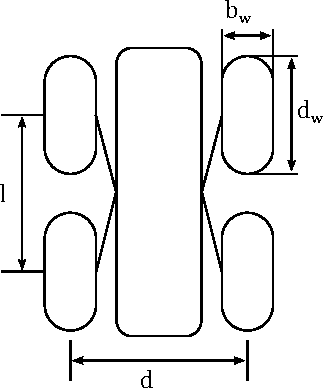
\includegraphics[width=0.7\textwidth]{Media/Geometries}
\caption{Geometric dimensions for the locomotion system.}
\label{fig:Ackerman}
}
\end{figure}

 
     
\begin{table}[htb]
     \centering
     \caption{Soil parameters for both soils considered: heav clay as hard equivalent for ice values and snow in Sweden \cite{Bekker}.}
     \begin{adjustbox}{max width=\textwidth}
     \begin{tabular}[l]{lcccccc}
     
     	\toprule
     		\multicolumn{1}{l}{Terrain} & \qquad \qquad	& \multicolumn{1}{c}{\(n\) /\(\frac{\text{kN}}{\text{m}^{n+1}}\)} & \multicolumn{1}{c}{\(k_\text{c}\)} & \multicolumn{1}{c}{\(k_\phi\) / \(\frac{\text{kN}}{\text{m}^{n+2}}\)} & \multicolumn{1}{c}{\(c\) /kPa} & \multicolumn{1}{c}{\(\phi\) /deg}  \\
      
       	\midrule
 
     Heavy Clay		&	&	0.13	&	12.70	&	1555.95		&	68.95	&	34			\\	
     Snow (Sweden)	&	&	1.44	&	10.55	&	66.08		&	6		&	20.7		\\	

     	\bottomrule
     
     \end{tabular}
     \end{adjustbox}
     \label{tab:SoilParam}
     \end{table}     


\begin{table}[htb]
\centering
\caption{Various wheel dimensions respective to the weight. Highlighted fields in red are not considered further for system design due to the limit of 200 g weight per wheel.}
\begin{adjustbox}{max width=\textwidth}
\begin{tabular}[l]{lcc|lcc}

	\toprule
		\multicolumn{1}{l}{Wheel Width} & \multicolumn{1}{c}{Wheel Diameter} & \multicolumn{1}{c|}{Weight per Wheel}	& \multicolumn{1}{l}{Wheel Width}	 & \multicolumn{1}{c}{Wheel Diameter} 		& \multicolumn{1}{c}{Weight per Wheel}    \\

\multicolumn{1}{l}{\:\:\:\:\:\: m}		& \multicolumn{1}{c}{m} 			& \multicolumn{1}{c|}{g} 					& \multicolumn{1}{l}{\:\:\:\:\:\: m}& \multicolumn{1}{c}{m}					& \multicolumn{1}{c}{g} \\
	\midrule
	
	0.05	&	0.1		&	127		& 0.05		&	0.15	&	185									\\ 
	0.06	&	0.1		&	153		&	0.06	&	0.15	&	\cellcolor[HTML]{CB0000}221		\\	
	0.07	&	0.1		&	178		&	0.07	&	0.15	&	\cellcolor[HTML]{CB0000}258		\\
	0.08	&	0.1		&	\cellcolor[HTML]{CB0000}204	&	0.08	&	0.15	&	\cellcolor[HTML]{CB0000}294		\\	
	0.09	&	0.1		&	\cellcolor[HTML]{CB0000}229	&	0.09	&	0.15	&	\cellcolor[HTML]{CB0000}331		\\
	0.1		&	0.1		&	\cellcolor[HTML]{CB0000}265	&	0.1		&	0.15	&	\cellcolor[HTML]{CB0000}367		\\	
	0.05	&	0.125	&	154		&	0.05	&	0.2		&	\cellcolor[HTML]{CB0000}236		\\
	0.06	&	0.125	&	185		&	0.06	&	0.2		&	\cellcolor[HTML]{CB0000}284		\\
	0.07	&	0.125	&	\cellcolor[HTML]{CB0000}217		&	0.07	&	0.2		&	\cellcolor[HTML]{CB0000}332		\\	
	0.08	&	0.125	&	\cellcolor[HTML]{CB0000}247		&	0.08	&	0.2		&	\cellcolor[HTML]{CB0000}379		\\
	0.09	&	0.125	&	\cellcolor[HTML]{CB0000}278		&	0.09	&	0.2		&	\cellcolor[HTML]{CB0000}427		\\
	0.1		&	0.125	&	\cellcolor[HTML]{CB0000}309		&	0.1		&	0.2		&	\cellcolor[HTML]{CB0000}487		\\
	
	\bottomrule

\end{tabular}
\end{adjustbox}
\label{tab:Geometry}
\end{table}


\subsubsection*{Mean Maximum Pressure}
\label{app:MMP}

To determine the mean maximum pressure, the data are taken from \autoref{fig:MMP_param}. 

\begin{figure}[htb] 
  \centering
     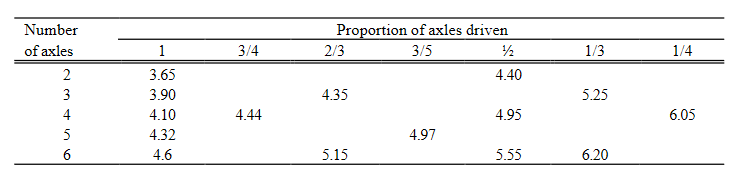
\includegraphics[width=1\textwidth]{Media/MMP_Param.png}
  \caption{Parameters for the mean maximum pressure for a wheeled rover.}
  \label{fig:MMP_param}
\end{figure}

The rover has 4 number ox axles, each with a quarter proportion of axles driven. Thus, the \(MMP\) can be calculated to:
\begin{equation}
	MMP \:  = \: \frac{K \cdot W}{2N{b_\text{w}}^{0.85}{d_\text{w}}^{1.15} { \left( \delta / d_\text{w} \right) }^{0.5}}		,
	\label{eq:MMP}
\end{equation}

with \(K = 6.05\) and the number of wheels \(N=4\). The resulting \(MMP\) for the 6 considered configurations are shown in \autoref{fig:MMP}. 

\begin{figure}[htb] 
  \centering
     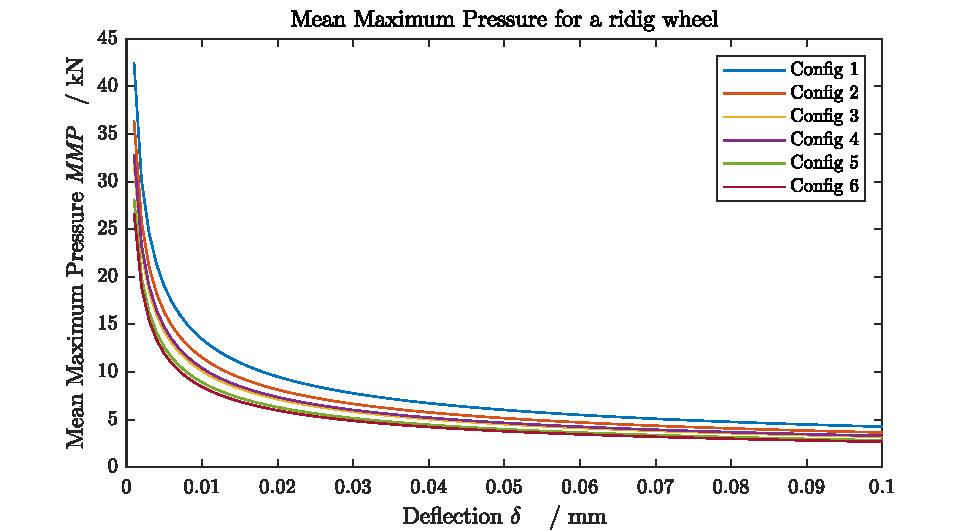
\includegraphics[width=1\textwidth]{Media/MMP for each Config.pdf}
  \caption{}
  \label{fig:MMP}
\end{figure}


\subsubsection*{Ackerman Steering}
\label{app:Ackerman}

As mentioned in \autoref{sec:Steering}, with Ackerman steering it is important to take into account that the angles of the front wheel positions differ: 

\begin{equation}
	\cot \theta_{i} - \cot \theta_\text{o} \:  = \:	- \frac{d}{l}	.
	\label{eq:Ackerman}
\end{equation}

With a wheel distance of \(d = 277\)~mm and \(l = 365\)~mm, the respective angles of the wheel positions can be determined. These values are necessary to control the drive in an autonomous drive mode.


\subsubsection*{Hardware Selection}
\label{app:Hardware}

Each wheel has a separate BLDC motor for driving. The necessary torque is listed for both soil parameters depending on the slope angle. In addition, necessary power is listed for different velocities to be reached, also for both soils. It should be noted, that the deflection \(\delta\) is not considered and assumed to be \(\delta = 0\).

\begin{table}[htb]
\centering
\caption{}
\begin{adjustbox}{max width=\textwidth}
\begin{tabular}[l]{lcccc|ccc}

	\toprule
		\multicolumn{1}{l}{\(\theta\)} & \multicolumn{1}{c}{\(R_\text{total,Snow}\)} & \multicolumn{1}{c}{\(\tau_\text{snow}\)} & \multicolumn{1}{c}{\(R_\text{total,HeavyClay}\)} & \multicolumn{1}{c|}{\(\tau_\text{HeavyClay}\)}	& \multicolumn{1}{c}{\(v\)}  & \multicolumn{1}{c}{\(P_\text{Min.,Snow}\)}  & \multicolumn{1}{c}{\(P_\text{Min.,HeavyClay}\)}			 \\
		
	\multicolumn{1}{l}{\:\:\:\:\:\: deg} & \multicolumn{1}{c}{N} & \multicolumn{1}{c}{Nm} & \multicolumn{1}{c}{N} & \multicolumn{1}{c|}{Nm} & \multicolumn{1}{c}{\(\frac{m}{s}\)} & \multicolumn{1}{c}{W} & \multicolumn{1}{c}{W} \\

	\midrule
		
	0	&	4.882	&	0.244	&	0.234	&	0.012	&	0.2		&	0.976	&	0.047	\\		
	7	&	6.040	&	0.302	&	1.436	&	0.072	&	0.35	&	2.114	&	0.503	\\
	14	&	7.094	&	0.355	&	2.618	&	0.131	&	0.5		&	3.547	&	1.309	\\
	21	&	8.028	&	0.401	&	3.765	&	0.188	&	0.65	&	5.219	&	2.447	\\
	28	&	8.833	&	0.442	&	4.857	&	0.243	&	0.8		&	7.067	&	3.886	\\
	35	&	9.499	&	0.475	&	5.880	&	0.294	&	0.95	&	9.024	&	5.586	\\
	
	\bottomrule

\end{tabular}
\end{adjustbox}
\label{tab:TorquePower}
\end{table}







\clearpage

\setcounter{figure}{0}
\setcounter{table}{0}

%-------------------------------------------------
\section{Electrical Power System} \label{sec:AppendixEPS}
%-------------------------------------------------
\begin{table}[htb]
\centering
\caption{INSPIRE battery parameters.}
\begin{tabular}{|c|c|}
\hline
\multicolumn{2}{|c|}{\textbf{SAFT 176065 xlr} \cite{SAFTBatteries.2018}}                                                                \\ \hline
\multicolumn{2}{|c|}{\textbf{Configuration:}}                                                                 \\ \hline
Battery Configuration                                                           & $3s4p$                        \\ \hline
Cells in Sereis $s$ N [-]                                                       & $3$                           \\ \hline
Cells in Parallel $p$ M [-]                                                     & $4$                           \\ \hline
\multicolumn{2}{|c|}{\textbf{Cell Parameters:}}                                                               \\ \hline
Typical Cell Capacity   [Ah]                                                    & $6.8$                         \\ \hline
Nominal Cell Voltage [V]                                                        & $3.65$                        \\ \hline
Nominal Cell Capacity [Wh]                                                      & $24.8$                        \\ \hline
Typical Cell Mass [kg]                                                          & $0.15$                        \\ \hline
Energy Density [Wh/kg]                                                     & $165.33$                      \\ \hline
\multicolumn{2}{|c|}{\textbf{Actual Battery Configuration Parameters:}}                                       \\ \hline
Battery Voltage $V_\text{Batt}$ [V]                                             & $10.95$                        \\ \hline
Battery Nominal Capacity $E_\text{Batt}$ [Wh]                                   & $297.6$                       \\ \hline
Battery Mass  [$kg$]                                                               & $1.8$                         \\ \hline
\textbf{Battery Mass} $m_\text{Batt}$ (incl. $10\%$ Margin) [kg]                                         & \textbf{1.98}                        \\ \hline
\multicolumn{2}{|c|}{\textbf{Configruation according to ECSS reliability restrictions and margins included:}} \\ \hline
Battery Configuration                                                           & $3s3p$                        \\ \hline
Cells in Sereis $s$ N [-]                                                       & $3$                           \\ \hline
Cells in Parallel $p$ M [-]                                                     & $3$                           \\ \hline
Battery Voltage $V_\text{Batt}$ [V]                                             & $10.95$                       \\ \hline
Battery Nominal Capacity $E_\text{Batt}$ [Wh]                                   & $231.60$                       \\ \hline
$30\%$ Margin on Energy Content                                                 & $0.3$                         \\ \hline
\textbf{Battery Nominal Capacity} $E_\text{Batt}$ incl. Margin [Wh]                      & \textbf{156.24}                      \\ \hline
Useable Energy Density [Wh/kg]                                              & $78.91$                       \\ \hline
\end{tabular}
\label{tab:battery}
\end{table}

\begin{figure}[htb]
{\centering
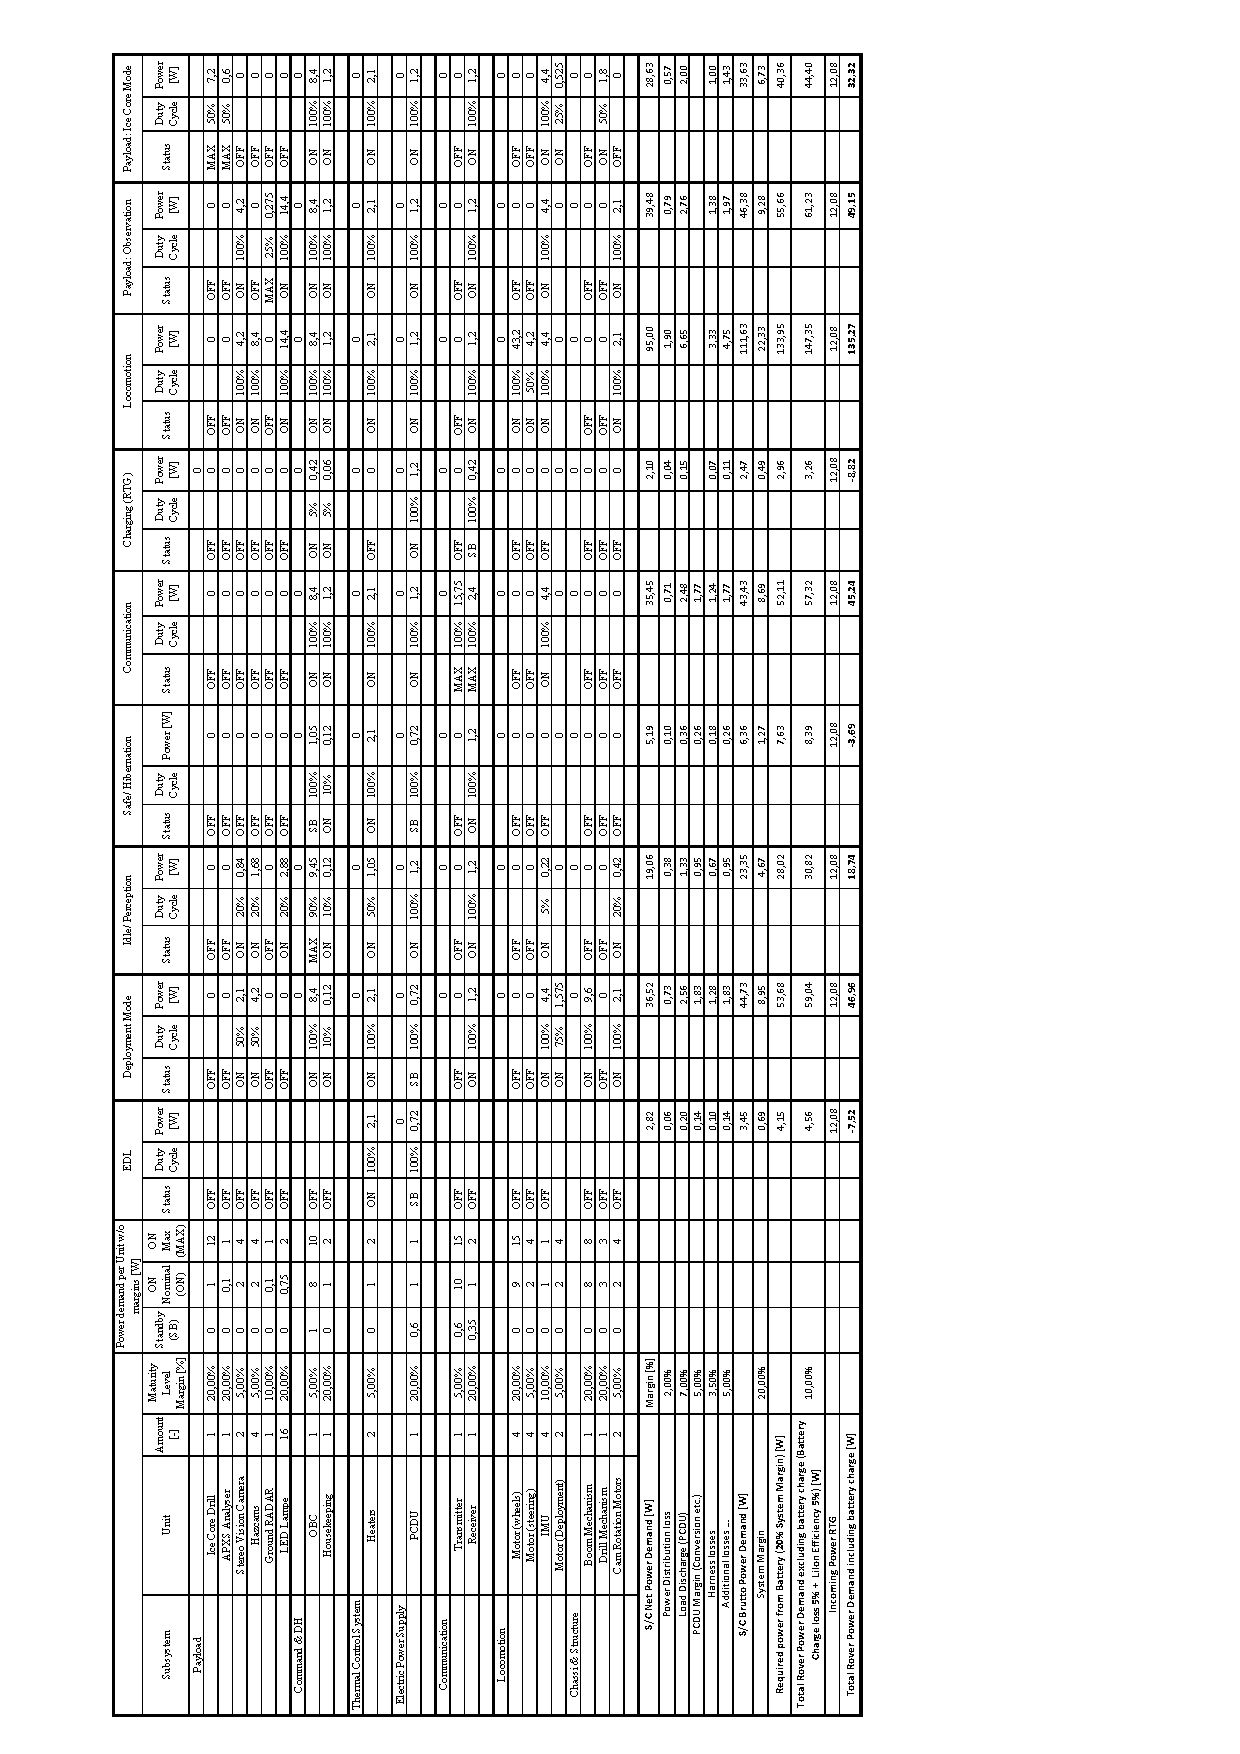
\includegraphics[width=1.0\textwidth]{Media/budgeteps}
\caption{Holistic Power Budget of INPSIRE.}
\label{tab:powerbudgetcomplete}
}
\end{figure}

\clearpage

\setcounter{figure}{0}
\setcounter{table}{0}

%-------------------------------------------------
\section{Communications} 
\label{sec:AppendixCOM}
%-------------------------------------------------

\subsection{Link Budget}
\label{app:LinkBudget}

Link budget considerations are performed under the conservative assumptions listed in \autoref{tab:lb-param}. \\

\begin{table}[h]
\centering
\begin{tabular}{llclll}
\hline
Parameter                        & Value  & Unit	       & Symbol        & Source                       &  \\ \hline
Rover                            &        &            &               &                              &  \\ \hline\hline
antenna Gain           		     & 2      & {[}dB{]}   & ${G}_{R}$  	   & omnidirectional LGA          &  \\
output power        	         & 1      & {[}W{]}    & ${P}_{R}$  	   & Digital Appendix                            &  \\
line loss               	     & 0,6    & {[}dB{]}   & ${L}_{l1}$ 	   & \cite{FLP_Exercise}                          &  \\ \hline
Path                             &        &            &               &                              &  \\ \hline\hline
R2L polarisation loss            & 0,3    & {[}dB{]}   & ${L}_{p}$ 	   & \cite{FLP_Exercise}                          &  \\
free space loss                  & 117,55 & {[}$m^3${]}& ${L}_{s}$  	   & \autoref{eqn:Ls}                             &  \\
atmospheric loss                 & 0      & {[}dB{]}   & ${L}_{a}$	   & negligible atmosphere        &  \\ \hline
Lander                           &        &            &               &                              &  \\ \hline\hline
antenna Gain             		 & 1      & {[}dB{]}   & ${G}_{L}$	   & conservative estimation      &  \\
output power        	         & 5      & {[}W{]}    & ${P}_{L}$  	   & conservative estimation      &  \\
pointing Loss  		             & 0      & {[}dB{]}   & ${n/a}$       & omnidirectional LGA          &  \\
line Loss  		                 & 0,6    & {[}dB{]}   & ${L}_{l2}$	   & \cite{FLP_Exercise}                          &  \\
eff. noise temperature           & 300    & {[}K{]}    & ${T}_{s}$	   & worst case E-bay temperature &  \\ \hline
Demodulation \& Uncertain Losses &        &            &               &                              &  \\ \hline\hline
eff. data rate                   & 5000   & {[}kbps{]} & ${R}$         & 50 \% of max. data rate                            &  \\
FEC coding                       & none   & {[}-{]}    & ${n/a}$       &  ${n/a}$                            &  \\
technical degradation            & 1      & {[}dB{]}   & ${L}_{i1}$    & \cite{FLP_Exercise}                          &  \\
implementation loss              & 1      & {[}dB{]}   & ${L}_{i1}$	   & \cite{FLP_Exercise}                          &  \\
                                 &        &            &               &                              & 
\end{tabular}
\caption{Transmission link parameters}
\label{tab:lb-param}
\end{table}

The free space loss ${L}_{s}$ [$m^3$] in \autoref{tab:lb-param} is calculated using the following correlation. 

\begin{equation}
	\centering
		{L}_{s} = {\frac{(4 \pi s)^2 \cdot c}{f}}
	\label{eqn:Ls}
\end{equation}

The signal travel distance {s} is assumed to be $s = 2000\ m$ which is in excess of the mission goal described in \autoref{chap:sc-output}. In accordance with X-Band communication the frequency {f} is set to a value of $f = 8,2\ GHz$. The parameter c represents the speed of light in vacuum. For simplification purposes $c = 3 \cdot 10^9\ \frac{m}{s}$ is assumed. \\ \\   
Combining the parameters from \autoref{tab:lb-param} the link budget is calculated using \autoref{eqn:EbzuN0}. For the simplification of \autoref{eqn:EbzuN0} the line losses for the rover ${L}_{l1}$ and lander ${L}_{l2}$ are expressed as the sum ${L}_{l}$. In the same manner technical degradation and implementation losses are combined to ${L}_{i}$. Atmospheric losses ${L}_{a}$ and pointing errors in \autoref{eqn:EbzuN0} are neglected due to a lack of atmosphere and the utilisation of omnidirectional low gain antennas. Parameter ${k}$ describes the Boltzmann constant.   

\begin{equation}
  \centering
		{\frac{{E}_{b}}{{N}_{0}}} = {P} - {L}_{l} + {G}_{R} - {10\cdot \log{{L}_{s}}} - {L}_{a} + {G}_{L} + {10\cdot \log{k}} - {10\cdot \log{{T}_{s}}} - {10\cdot \log{{R}}} - {L}_{i}
	\label{eqn:EbzuN0}
\end{equation}


\autoref{eqn:EbzuN0} and the conservative assumptions from \autoref{tab:lb-param} results in an energy per bit over noise $\frac{{E}_{b}}{{N}_{0}} = 10,59\ dB$. The complete link budget can be found in \autoref{fig:LB-R2L}. \\
Referencing \autoref{fig:BitErrorRate} a Bit Error Rate of $10^{-4}$ can be achieved in the downlink path, which is considered sufficient for a first assessment. Optionally a FEC code can be implemented in later design phases.\\

Using the same parameters listed in \autoref{tab:lb-param} leads to a $\frac{{E}_{b}}{{N}_{0}} = 50,56\ dB$ corresponding to a Bit Error Rate of potentially less than $10^{-6}$. Therefore the downlink does not contribute to the design decisions. The complete link budget for the uplink path can be found in \autoref{fig:LB-L2R}.

%Complete Link Budget for Rover to Lander Transmission
\begin{table}[]
\centering
\caption{Complete link budget for Rover to Lander transmission.}
\label{tab:lb-R2L}
\begin{tabular}{llll}
\multicolumn{4}{l}{Rover to Lander (R2L) Link Budget (uplink)}                   \\ \hline
\multicolumn{4}{l}{\cellcolor[HTML]{DAE8FC}Rover}                                \\
Rover transmitter output power            &${P}_{R}$		& 1                      & W    \\
                                          &${P}_{R}$    & 0                      & dB   \\
Rover line loss                           &${L}_{l1}$   & 0.6                    & dB   \\
Rover antenna gain                        &${G}_{R}$ 	& 2                      & dB   \\
\multicolumn{4}{l}{\cellcolor[HTML]{DAE8FC}Downlink Path}                        \\
Rover antenna pointing loss               &n/a    		& 0                      & dB   \\
polarization loss                     	  &${L}_{p}$		& 0.3                    & dB   \\
free space loss                           &${L}_{s}$		& 116.74                 & dB   \\
atmospheric loss                          &${L}_{a}$		& 0                      & dB   \\ \hline
signal level at Lander                    &RIP      		& -115.64                & dB   \\
\multicolumn{4}{l}{\cellcolor[HTML]{DAE8FC}Lander}                               \\
Lander LGA pointing loss                  &      		& 0                      & dB   \\
Lander antenna gain                       &${G}_{L}$		& 1                      & dB   \\ \hline
signal after Lander LGA                   &      		& -114.64                & dB   \\ \hline
Lander line loss                    		  &${L}_{l2}$	& 0.6                    & dB   \\
Lander effective noise temp.              &${T}_{s}$ 	& 24.77                  & dB   \\ \hline
Lander signal to noise power density      & $\frac{C}{{N}_{0}}$ & 88.58                  & dB   \\ \hline
\multicolumn{4}{l}{\cellcolor[HTML]{DAE8FC}Data Rate}                            \\ \hline
data rate                                 &${R}$			& 5000                   & kbps \\
                                          &${R}$			& -66.99                 & dBHz \\ \hline
\multicolumn{4}{l}{\cellcolor[HTML]{DAE8FC}Total}                                \\ \hline
System $\frac{{E}_{b}}{{N}_{0}}$ for L2R link &$\frac{{E}_{b}}{{N}_{0}}$& 21.59                  & dB   \\
\multicolumn{4}{l}{}                                                             \\ \hline
\multicolumn{4}{l}{\cellcolor[HTML]{DAE8FC}Demodulation}                         \\ \hline
specified Bit Error Rate                  &BER      		& $10^{-4}$ 				 & n/a  \\
FEC coding used                           &      		& none                   &      \\
$\frac{{E}_{b}}{{N}_{0}}$ threshold       &      		& 9                      & dB   \\ \hline
\multicolumn{4}{l}{\cellcolor[HTML]{DAE8FC}Uncertain Losses}                     \\ \hline
technical degradation                     &${L}_{i1}$	& 1                      & dB   \\
implementation loss                       &${L}_{i2}$	& 1                      & dB   \\
\multicolumn{4}{l}{}                                                             \\ \hline
\multicolumn{4}{l}{\cellcolor[HTML]{DAE8FC}Link Margin}                          \\ \hline
system link margin after uncertain losses &$\frac{{E}_{b}}{{N}_{0}}$& 10.59                  & dB  
\end{tabular}
\end{table}

%Complete Link Budget for Lander to Rover Transmission
\begin{table}[]
\centering
\caption{Complete link budget for Lander to Rover (L2R) transmission.}
\label{tab:lb-L2R}
\begin{tabular}{llll}
\multicolumn{4}{l}{Lander to Rover (L2R) Link Budget (downlink)}                 \\ \hline
\multicolumn{4}{l}{\cellcolor[HTML]{DAE8FC}Lander}                               \\
Lander transmitter output power           &${P}_{L}$		& 5                      & W    \\
                                          &${P}_{L}$		& 6.99                   & dB   \\
Lander line loss                          &${L}_{l2}$	& 0.6                    & dB   \\
Lander antenna gain                       &${G}_{L}$		& 1                      & dB   \\
\multicolumn{4}{l}{\cellcolor[HTML]{DAE8FC}Uplink Path}                          \\
pointing loss                             &n/a	    		& 0                      & dB   \\
polarization loss                         &${L}_{p}$		& 0.3                    & dB   \\
free space loss                           &${L}_{s}$		& 116.74                 & dB   \\
atmospheric loss                          &${L}_{a}$		& 0                      & dB   \\ \hline
signal level at Lander					  & RIP  & 109.65				  & dB   \\ 
\multicolumn{4}{l}{\cellcolor[HTML]{DAE8FC}Rover}                                \\
Rover LGA pointing loss                   &n/a	    		& 0                      & dB   \\
Rover antenna gain                        &${G}_{R}$		& 1                      & dB   \\ \hline
signal after Rover LGA                    &      		& 108.65                 & dB   \\ \hline
Rover line loss                     	      &${L}_{l1}$	& 0.6                    & dB   \\
Rover effective noise temp.               &${T}_{s}$ 	& 24.77                  & dB   \\ \hline
Rover signal to noise power density       & $\frac{C}{{N}_{0}}$	 & 94.57                  & dB   \\ \hline
\multicolumn{4}{l}{\cellcolor[HTML]{DAE8FC}Data Rate}                            \\ \hline
data rate                                 &${R}$   		& 2                      & kbps \\
                                          &${R}$ 		& 33.01                  & dBHz \\ \hline
\multicolumn{4}{l}{\cellcolor[HTML]{DAE8FC}Total}                                \\ \hline
System $\frac{{E}_{b}}{{N}_{0}}$for L2R link &      		& 61.56                  & dB   \\
\multicolumn{4}{l}{}                                                             \\ \hline
\multicolumn{4}{l}{\cellcolor[HTML]{DAE8FC}Demodulation}                         \\ \hline
specified Bit Error Rate                  &BER      		& $10^{-6}$ 			  & n/a  \\
FEC coding used                           &      		& none                   &      \\
$\frac{{E}_{b}}{{N}_{0}}$ threshold       &				& 11                     & dB   \\ \hline
\multicolumn{4}{l}{\cellcolor[HTML]{DAE8FC}Uncertain Losses}                     \\ \hline
technical degradation                     &${L}_{i1}$	& 1                      & dB   \\
implementation loss                       &${L}_{i1}$	& 1                      & dB   \\
\multicolumn{4}{l}{}                                                             \\ \hline
\multicolumn{4}{l}{\cellcolor[HTML]{DAE8FC}Link Margin}                          \\ \hline
system link margin after uncertain losses &$\frac{{E}_{b}}{{N}_{0}}$	& 48.56      & dB  
\end{tabular}
\end{table}

\begin{figure}[h]
	\centering
  		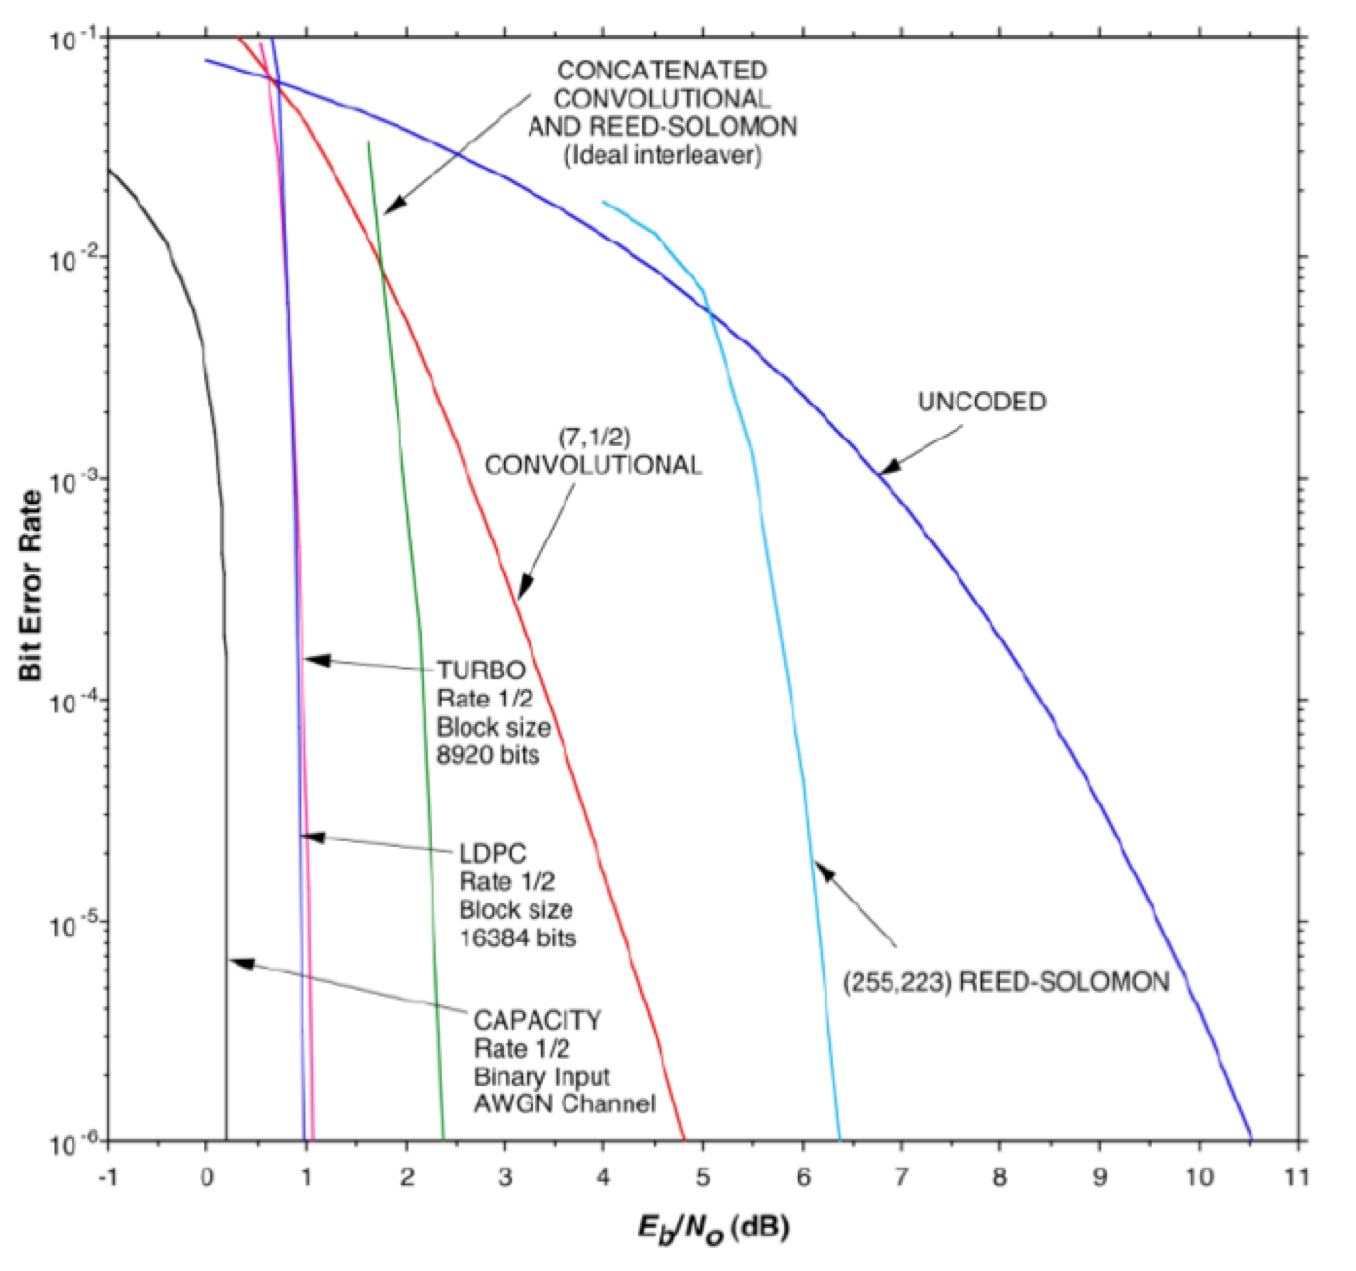
\includegraphics[width=0.5\textwidth]{Media/Bit_Error_Rate.png}
  \caption{Bit Error Rate for different FEC codes}
  \label{fig:BitErrorRate}
\end{figure}

\subsection{Mission Data Output}
\label{app:MissionDataOutput}

The analysis of the mission data concept for memory capacity and transmission times is focuses on the payload camera and Hazcams as images require far more data than telemetry or other payload data. \\

In a first assumption 420 images per day are stored and transmitted. Considering the sensor resolution of $2048\times2048$ pixels and a bit depth per pixel of 10 bit of the (CAMERA REFERENCE), a file size of 42 Mbit per image is assumed.\\
To calculate the message size in \autoref{tab:TimePerPic}, it is assumed that a transmission frame consists of 10264 bits including a payload frame of maximum 8840 bits (FLP VORELESUNG).   

\begin{table}[h]
\centering
\begin{tabular}{llllll}
File Type & Compression    & File Size  & Message Size & Data Rate & Tx t per File \\ \hline\hline
image     & none           & 42 Mbit    & 48,77 Mbit   & 5 Mbit    & 8,12 s        \\
image     & HIREW          & 23,52 Mbit & 27,31 Mbit   & 5 Mbit    & 5,45 s        \\ \hline
\end{tabular}
\caption{Comparison of transmission times per image (message frame bits included)}
\label{tab:TimePerPic}
\end{table}

\begin{table}[h]
\centering
\begin{tabular}{lllll}
File per tal & Compression & File Size  & Total Data & Tx time    \\ \hline\hline
420          & none        & 42 Mbit    & 2,21 GB    & 56,9 Min.  \\
420          & HIREW       & 23,52 Mbit & 1,22 GB    & 38,23 Min. \\ \hline
\end{tabular}
\caption{Transmission time and total data output per mission day}
\label{tab:Tx-tptal}
\end{table}

The HIREW compression algorithm is suggested for the mission considering a high average compression of 0,56 \% and a high compression speed of 123 Mbit/s for grayscale and 104,4 Mbit/s for RGB image files \cite{HIREW}. 

\subsection{Communications Trade Off}
\label{app:Com_TrOff}

\subsubsection{Transmitter Selection}
% Transmitter Trade off
\begin{figure}[h]
     \centering
     \begin{subfigure}[b]{0.49\textwidth}
         \centering
         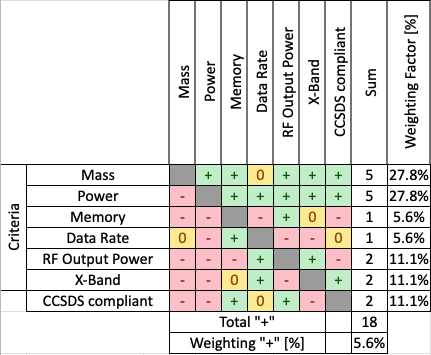
\includegraphics[width=\textwidth]{Media/Trade_off/Transmitter/Weighting_trans.png}
         \caption{Weighting of selection criteria for the transmitter.}
         \label{fig:Weighting_trans}
     \end{subfigure}
     \hfill
     \begin{subfigure}[b]{0.49\textwidth}
         \centering
         \includegraphics[width=\textwidth]{Media/Trade_off/Transmitter/Values_trans.png}
         \caption{Comparison of optional transmitters.}
         \label{fig:Values_trans}
     \end{subfigure}
     \hfill
     \begin{subfigure}[b]{0.49\textwidth}
         \centering
         \includegraphics[width=\textwidth]{Media/Trade_off/Transmitter/TradeOff_trans.png}
         \caption{Transmitter trade off.}
         \label{fig:TradeOff_trans}
     \end{subfigure}
     \hfill
     \caption{Transmitter Trade off for the Communication subsystem.}
     \label{TrOff_Trans}
\end{figure}

\subsubsection{Receiver Trade Off}
%Receiver Trade Off
\begin{figure}[h]
     \centering
     \begin{subfigure}[b]{0.49\textwidth}
         \centering
         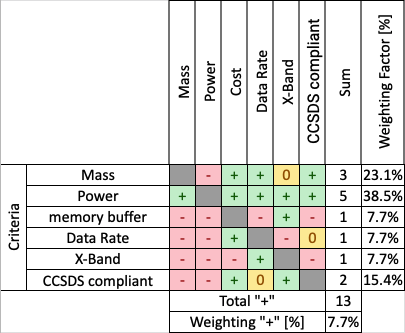
\includegraphics[width=\textwidth]{Media/Trade_off/Receiver/Weighting_Rec.png}
         \caption{Weighting of selection criteria for the receiver.}
         \label{fig:Weighting_Rec}
     \end{subfigure}
     \hfill
     \begin{subfigure}[b]{0.49\textwidth}
         \centering
         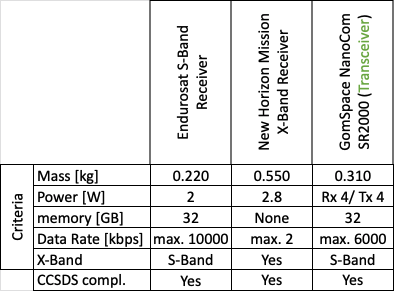
\includegraphics[width=\textwidth]{Media/Trade_off/Receiver/Values_Rec.png}
         \caption{Comparison of optional receivers.}
         \label{fig:Values_Rec}
     \end{subfigure}
     \hfill
     \begin{subfigure}[b]{0.49\textwidth}
         \centering
         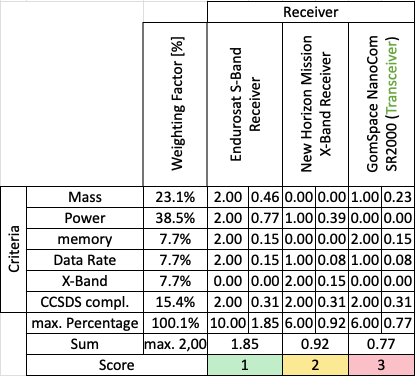
\includegraphics[width=\textwidth]{Media/Trade_off/Receiver/TradeOff_Rec.png}
         \caption{Receiver trade off.}
         \label{fig:TradeOff_Rec}
     \end{subfigure}
     \hfill
     \caption{Receiver Trade off for the Communication subsystem.}
     \label{TrOff_Trans}
\end{figure}

\subsubsection{Antenna Trade Off}
%Antenna Trade Off
\begin{figure}[h]
     \centering
     \begin{subfigure}[b]{0.49\textwidth}
         \centering
         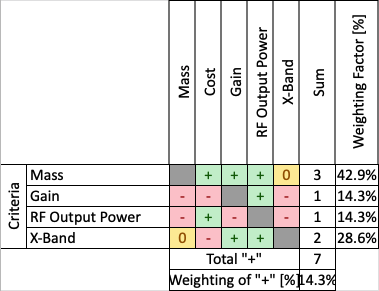
\includegraphics[width=\textwidth]{Media/Trade_off/Antenna/Weighting_Ant.png}
         \caption{Weighting of selection criteria for the antenna.}
         \label{fig:Weighting_Rec}
     \end{subfigure}
     \hfill
     \begin{subfigure}[b]{0.49\textwidth}
         \centering
         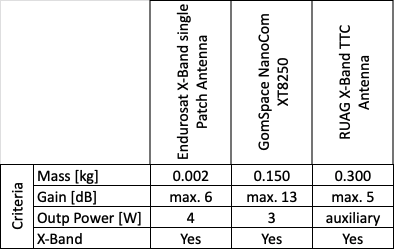
\includegraphics[width=\textwidth]{Media/Trade_off/Antenna/Values_Ant.png}
         \caption{Comparison of optional antenna.}
         \label{fig:Values_Rec}
     \end{subfigure}
     \hfill
     \begin{subfigure}[b]{0.49\textwidth}
         \centering
         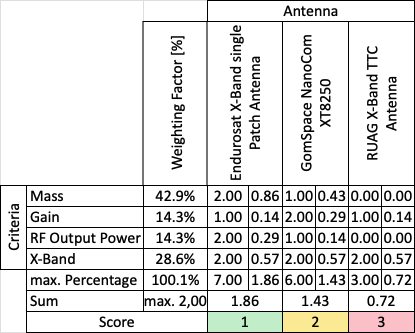
\includegraphics[width=\textwidth]{Media/Trade_off/Antenna/TradeOff_Ant.png}
         \caption{Antenna trade off.}
         \label{fig:TradeOff_Rec}
     \end{subfigure}
     \hfill
     \caption{Antenna trade off for the Communication subsystem.}
     \label{TrOff_Trans}
\end{figure}

\subsection{Command \& Data Handling Trade Off}

\subsubsection{OBC Trade Off}
%OBC Trade Off
\begin{figure}[htb]
     \centering
     \begin{subfigure}[b]{0.49\textwidth}
         \centering
         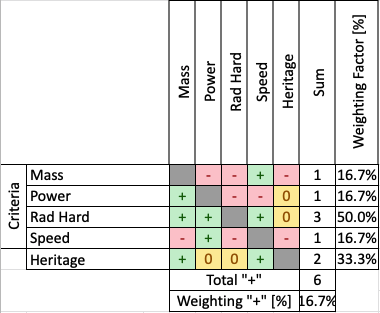
\includegraphics[width=\textwidth]{Media/Trade_off/OBC/Weighting_OBC.png}
         \caption{Weighting of selection criteria for the OBC.}
         \label{fig:Weighting_Rec}
     \end{subfigure}
     \hfill
     \begin{subfigure}[b]{0.49\textwidth}
         \centering
         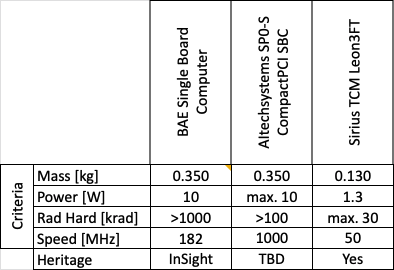
\includegraphics[width=\textwidth]{Media/Trade_off/OBC/Values_OBC.png}
         \caption{Comparison of optional single board computers.}
         \label{fig:Values_Rec}
     \end{subfigure}
     \hfill
     \begin{subfigure}[b]{0.49\textwidth}
         \centering
         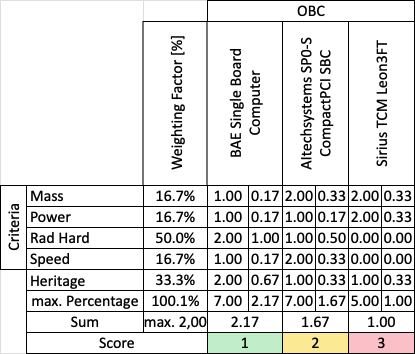
\includegraphics[width=\textwidth]{Media/Trade_off/OBC/TradeOff_OBC.png}
         \caption{Antenna trade off.}
         \label{fig:TradeOff_Rec}
     \end{subfigure}
     \hfill
     \caption{OBC trade off for the Command \& Data Handling subsystem.}
     \label{TrOff_Trans}
\end{figure}

\clearpage

\setcounter{figure}{0}
\setcounter{table}{0}

%-------------------------------------------------
\section{Thermal Controls System} \label{sec:AppendixThermal}
%-------------------------------------------------
\subsection{Results}
\begin{table}[htb]
	\centering
	\caption{Temperature results in K of thermal analysis, \textit{with out}  margin .}
	\begin{tabular}{lccccc}
		\toprule
		Components & Hot Case & Cold Case & Charging & Communication & Analyse  \\ \midrule
		RTG  & 415 & 391 & 402 & 407  &  401   \\
		Electric Bay & 301 & 268 & 293 & 313 & 28 \\
		Drill  & 283 & 256 & 267 & 271 & 328  \\
		Camera & 327 & 249 & 256 & 257 & 256 \\
		Chassis & 268 & 230  & 245 & 251 & 246 \\
		Steer Engine & 296 & 249 & 260 & 262 & 261  \\
		Drive Engine & 344 & 251 & 262 & 262 & 262 \\   \bottomrule
	\end{tabular}
	\label{tab:tcs_temp1}
\end{table}

\begin{table}[htb]
	\centering
	\caption{Temperature results in K of thermal analysis, \textit{with}  margin .}
	\begin{tabular}{lccccc}
		\hline
		Components & Hot Case & Cold Case & Charging & Communication & Analyse  \\[0.25em]
		Margin & +15~K & -15~K & +15~K & +15~K & +15~K \\ \hline
		RTG  & 430 & 376 & 417 & 422  & 416    \\
		Electric Bay & 316 & \cellcolor[HTML]{FFCE93} 253$^1)$ & 308 &\cellcolor[HTML]{FFCE93} 328$^1)$ & 296 \\
		Drill  & 298 & 241 & 282 & 286 & 343  \\
		Camera & 342 & 234 & 271 & 272 & 271 \\
		Chassis & 283 & 215 & 260 & 266 & 261 \\
		Steering Engine & 311 & 234 & 275 & 277 & 276  \\
		Drive Engine & 359 & 236 & 277 & 277 & 277 \\   \hline
		& & & & & \\[-0.5em]
		\multicolumn{6}{l}{$^1)$\ Exeeding transmitter temperature limits.}
	\end{tabular}
	\label{tab:tcs_temp2}
\end{table}



\subsection{Heat energy eqilibrium}  \label{sec:app_tcs_01}
The follwing equiations describe each node of the thermal network.
The input values were tanken from EPS, \autoref{sec:app_therm_2}, \autoref{sec:app_therm_3}, \autoref{sec:app_therm_4} respectively.

\begin{table}[H]
	\begin{tabular}{l@{\quad}l@{\qquad\qquad\qquad}l@{\quad}l}
		\multicolumn{4}{l}{\textit{Subscript} for eqilibrium:}\\[0.5em]
		Bay & Electrical Bay & D	& Drill\\
		Bo & Bogie & 	E,D & Drive Engine\\
		Cam & Camera & E,S & Steer Engine\\
		C & Chassis & WF & Wheel Fork\\
	\end{tabular}

\end{table}

\underline{RTG:}
\begin{equation}
\begin{aligned}
0=\  &\dot{Q}_{RTG} +CON_1 \cdot (T_{Bay}-T_{RTG})+CON_2 \cdot (T_{C}-T_{RTG})+ \\[1em]
& + CON_5 \cdot (T_{D}-T_{RTG})+ CON_9 \cdot (T_{E,S}-T_{RTG})\\[1em]
& +   CON_12 \cdot (T_{E,D}-T_{RTG}) - \epsilon_{RTG}\cdot \sigma_b \cdot S_{RTG}\cdot T_{RTG}^4 \\[2em]
\end{aligned}
\end{equation}

\underline{Electric Bay:}
\begin{equation}
	\begin{aligned}
		0=\ &  \dot{Q}_{Bay}+ CON_1 \cdot (T_{RTG}-T_{Bay})+ (CON_3+n_{S2}\cdot CON_{S2}) \cdot (T_{C}-T_{Bay})-\\[1em]
		&  -\epsilon_{Bay}\cdot \sigma_b \cdot S_{Bay}\cdot T_{Bay}^4
	\end{aligned}
\end{equation}\\
with: 
\begin{equation} \dot{Q}_{Bay} = \dot{Q}_{OBC} + \dot{Q}_{Tranceiver} +\dot{Q}_{Receiver} +\dot{Q}_{PCDU} \end{equation}\\

\underline{Drill \& Analyser:}
\begin{equation} 0= \ \dot{Q}_{D} +CON_4 \cdot (T_{C}-T_{D})+CON_5 \cdot (T_{RTG}-T_{D})   \end{equation} \\
%
\underline{Camera:}
\begin{equation}
\begin{aligned}
0=\  &  \dot{Q}_{Cam} + \dot{Q}_{RHU} +CON_6 \cdot (T_{C}-T_{Cam})+ \\[1em]
& +(CON_{14} +n_{S1}\cdot CON_{S1}) \cdot (T_{Rad}-T_{Cam})  -\\[1em]
& - \epsilon_{Cam}\cdot \sigma_b \cdot S_{Cam}\cdot T_{Cam}^4 \\[2em]
\end{aligned}
\end{equation}
%
\underline{Radiator:}
\begin{equation}0=(CON_{14} +n_{S1}\cdot CON_{S1}) \cdot (T_{Cam}-T_{Rad}) - \epsilon_{Rad}\cdot \sigma_b \cdot S_{Rad}\cdot T_{Rad}^4  \end{equation}  \\
%
\underline{Chassis:}
\begin{equation}
\begin{aligned}
0=\  &   \dot{Q}_{Radar}+\dot{Q}_{Hazcam} +\dot{Q}_{Analyser} +\dot{Q}_{IMUs} +\\[1em]
	& +CON_2 \cdot (T_{RTG}-T_{C})+(CON_3+n_{S2}\cdot CON_{S2})\cdot (T_{Bay}-T_{C})+ \\[1em]
&  +  CON_4 \cdot (T_{Drill}-T_{C})+CON_6 \cdot (T_{Cam}-T_{C})+CON_7 \cdot (T_{Node_1}-T_{C}) +  \\[1em]
&  + \alpha_{C}\cdot [ S_0 \cdot (1+\rho_E) \cdot (S_{Ch1} \cdot \varphi_1  +S_{Ch2} \cdot \varphi_2 ) +   \epsilon_{E} \cdot \sigma_b \cdot S_{Ch3}\cdot T_{Surface}^4 ]+  \\[1em]
& +\epsilon_{Bay}\cdot \sigma_b \cdot S_{Bay}\cdot T_{Bay}^4 - \frac{1}{2} \cdot \epsilon_{Bo}\cdot \sigma_b \cdot S_{Bo}\cdot \left( \frac{T_{C}}{2} +\frac{T_{Node_1}}{2}  \right)^4  -\epsilon_{C}\cdot \sigma_b \cdot S_{C}\cdot T_{C}^4 \\[2em]
\end{aligned}
\end{equation}

\underline{Steer Engine:}
\begin{equation}
\begin{aligned}
0=\  &  4\cdot [\dot{Q}_{E,S} +CON_8  \cdot (T_{Node1}-T_{E,S})+ \\[1em]
&   +CON_9 \cdot (T_{RTG}-T_{E,S}) -\epsilon_{E,S}\cdot \sigma_b \cdot S_{E,S}\cdot T_{E,S}^4] \\[2em]
\end{aligned}
\end{equation}

\underline{Distribution Node 1:}
\begin{equation}
\begin{aligned}
0=\  &  4\cdot [CON_7 \cdot (T_{C}-T_{Node_1})+CON_8 \cdot (T_{E,S}-T_{Node_1})+ \\[1em]
&   +CON_10 \cdot (T_{Node_2}-T_{Node_1}) - \\[1em]
&  - \frac{1}{2} \cdot \epsilon_{Bo}\cdot \sigma_b \cdot S_{Bo}\cdot \left( \frac{T_{C}}{2} +\frac{T_{Node_1}}{2}  \right)^4  - \\[1em]
& - \frac{1}{2} \cdot \epsilon_{WF}\cdot \sigma_b \cdot S_{WF}\cdot \left( \frac{T_{Node_1}}{2} +\frac{T_{Node_2}}{2}  \right)^4- \\[1em]
& -\epsilon_{E,S}\cdot \sigma_b \cdot S_{E,S}\cdot T_{E,S}^4\ ] \\[2em]
\end{aligned}
\end{equation}

\underline{Drive Engine:}
\begin{equation}
\begin{aligned}
0=\  &  4 \cdot [\dot{Q}_{E,D}+ (CON_{11}+n_{S3}\cdot CON_{S3}) \cdot (T_{Node_2}-T_{E,D})+ \\[1em]
&  + CON_{12} \cdot (T_{RTG}-T_{E,D})-\epsilon_{E,D}\cdot \sigma_b \cdot S_{E,D}\cdot T_{E,D}^4 ]  \\[2em]
\end{aligned}
\end{equation}

\underline{Distribution Node 2:}
\begin{equation}
\begin{aligned}
0=\ & 4 \cdot [CON_{10} \cdot (T_{Node_1}-T_{Node_2})+CON_{13} \cdot (T_{Ground}-T_{Node_2}) +   \\[1em]
&   +(CON_{11}+n_{S3}\cdot CON_{S3}) \cdot (T_{E,D}-T_{Node_2}) + \\[1em]
& - \frac{1}{2} \cdot \epsilon_{WF}\cdot \sigma_b \cdot S_{WF}\cdot \left( \frac{T_{Node_1}}{2} +\frac{T_{Node_2}}{2}  \right)^4- \\[1em]
& -\epsilon_{E,D}\cdot \sigma_b \cdot S_{E,D}\cdot T_{E,D}^4\ ] \\[2em]
\end{aligned}
\end{equation}
\clearpage

\subsection{Heat conductance} \label{sec:app_therm_2}

\begin{table}[htb]
	\centering
	\caption{Definition of heat conductance C between the nodes according to \autoref{fig:tcs_network}.}
	\begin{tabular}{l@{\qquad}cccc}
		\hline
		Name &  Linked Components &  \multicolumn{3}{c}{Geometry}\\ \hline
		& & & & \\[-0.75em]
		\textbf{Linkage} & \textbf{RTG} $\leftrightarrow$ \textbf{Chassis}  &  \multicolumn{3}{c}{\multirow{2}{*}{\adjustbox{valign=t}{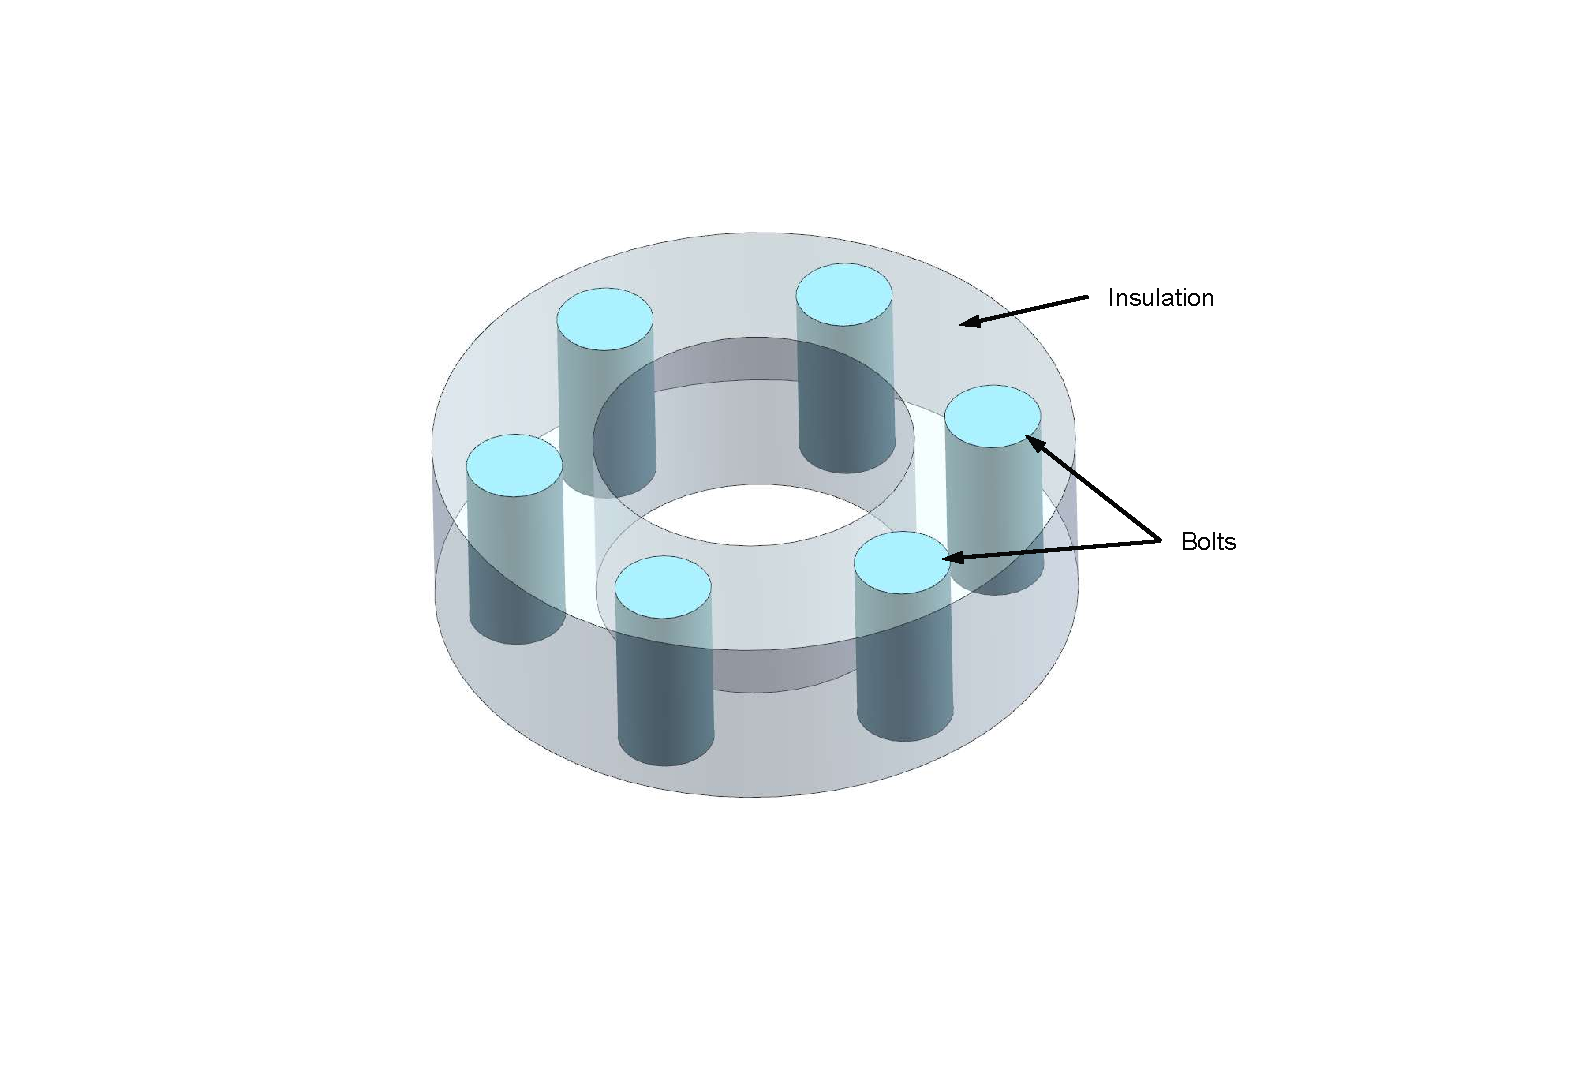
\includegraphics[width=0.3\textwidth]{Media/tcs_con_rtg}}}}  \\[1em]
		& & & &  \\
		\multicolumn{2}{l}{$CON_2= CON_{I}+n_{B}\cdot CON_{B}$} & & & \\[1em]
		\multicolumn{2}{l}{$CON_2= 1.50 \cdot 10^{-1}\ \frac{\W}{\K} $} & & &  \\[3em]
		\hline
		Part &  Cross section & Thickness  & Material & Amount \\ \hline
		& & & & \\[-0.75em]
		Insulation & $S_I=3'770\ \mm^2$ & $t_I=12\ \mm$ & Aerogel & 1 \\[0.5em]
		Bolts, M6 & $S_B=28.3\ \mm^2$ & $t_B=12\ \mm$ & Titan & 10 \\[5em]
		
		\hline
		Name &  Linked Components &  \multicolumn{3}{c}{Geometry}\\ \hline
		& & & & \\[-0.5em]
		\textbf{Linkage} & \textbf{EBay} $\leftrightarrow$ \textbf{Chassis}  &  \multicolumn{3}{c}{\multirow{2}{*}{\adjustbox{valign=t}{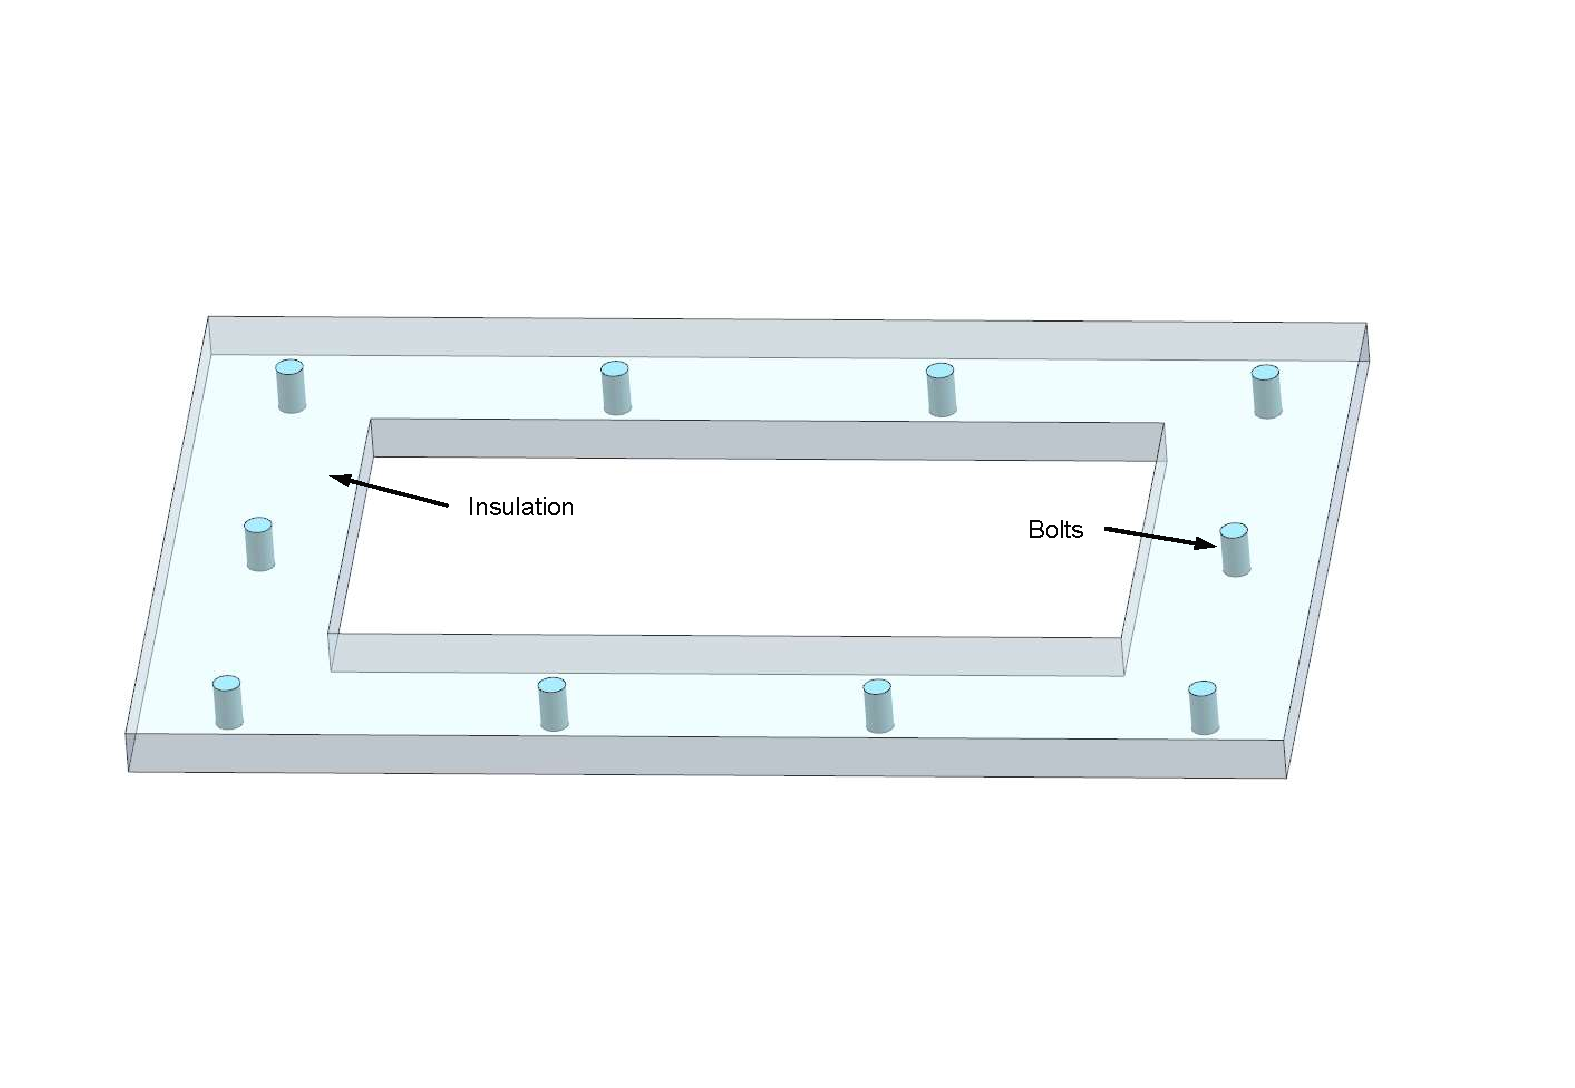
\includegraphics[width=0.5\textwidth]{Media/tcs_con_bay}}}}  \\[1em]
		& & & &  \\
		\multicolumn{2}{l}{$CON_3= CON_{I}+n_{B}\cdot CON_{B}$} & & &  \\[1em]
		\multicolumn{2}{l}{$CON_3= 4.20 \cdot 10^{-1}\ \frac{\W}{\K}$} & & & \\[3em]
		
		\hline
		Part &  Cross section & Thickness  & Material & Amount \\ \hline
		& & & & \\[-0.75em]
		Insulation & $S_I=27'120 \ \mm^2$ & $t_I=8\ \mm$ & Aerogel & 1 \\[0.5em]
		Bolts, M6 & $S_B=28.3 \ \mm^2$ & $t_B=8\ \mm$ & Titan & 10 \\	
	\end{tabular}
	\label{tab:tcs_nodes1}
\end{table}	

\begin{table}[htb]
	\centering
	\caption{Definition of heat conductance $CON=\frac{1}{R}$ between the nodes according to \autoref{fig:tcs_network}.}
	\begin{tabular}{l@{\qquad}cccc}
				\hline
		Name &  Linked Components &  \multicolumn{3}{c}{Geometry}\\ \hline
		& & & & \\[-0.5em]
		\textbf{Linkage} & \textbf{Drill} $\leftrightarrow$ \textbf{Chassis}  &  \multicolumn{3}{c}{\multirow{2}{*}{\adjustbox{valign=t}{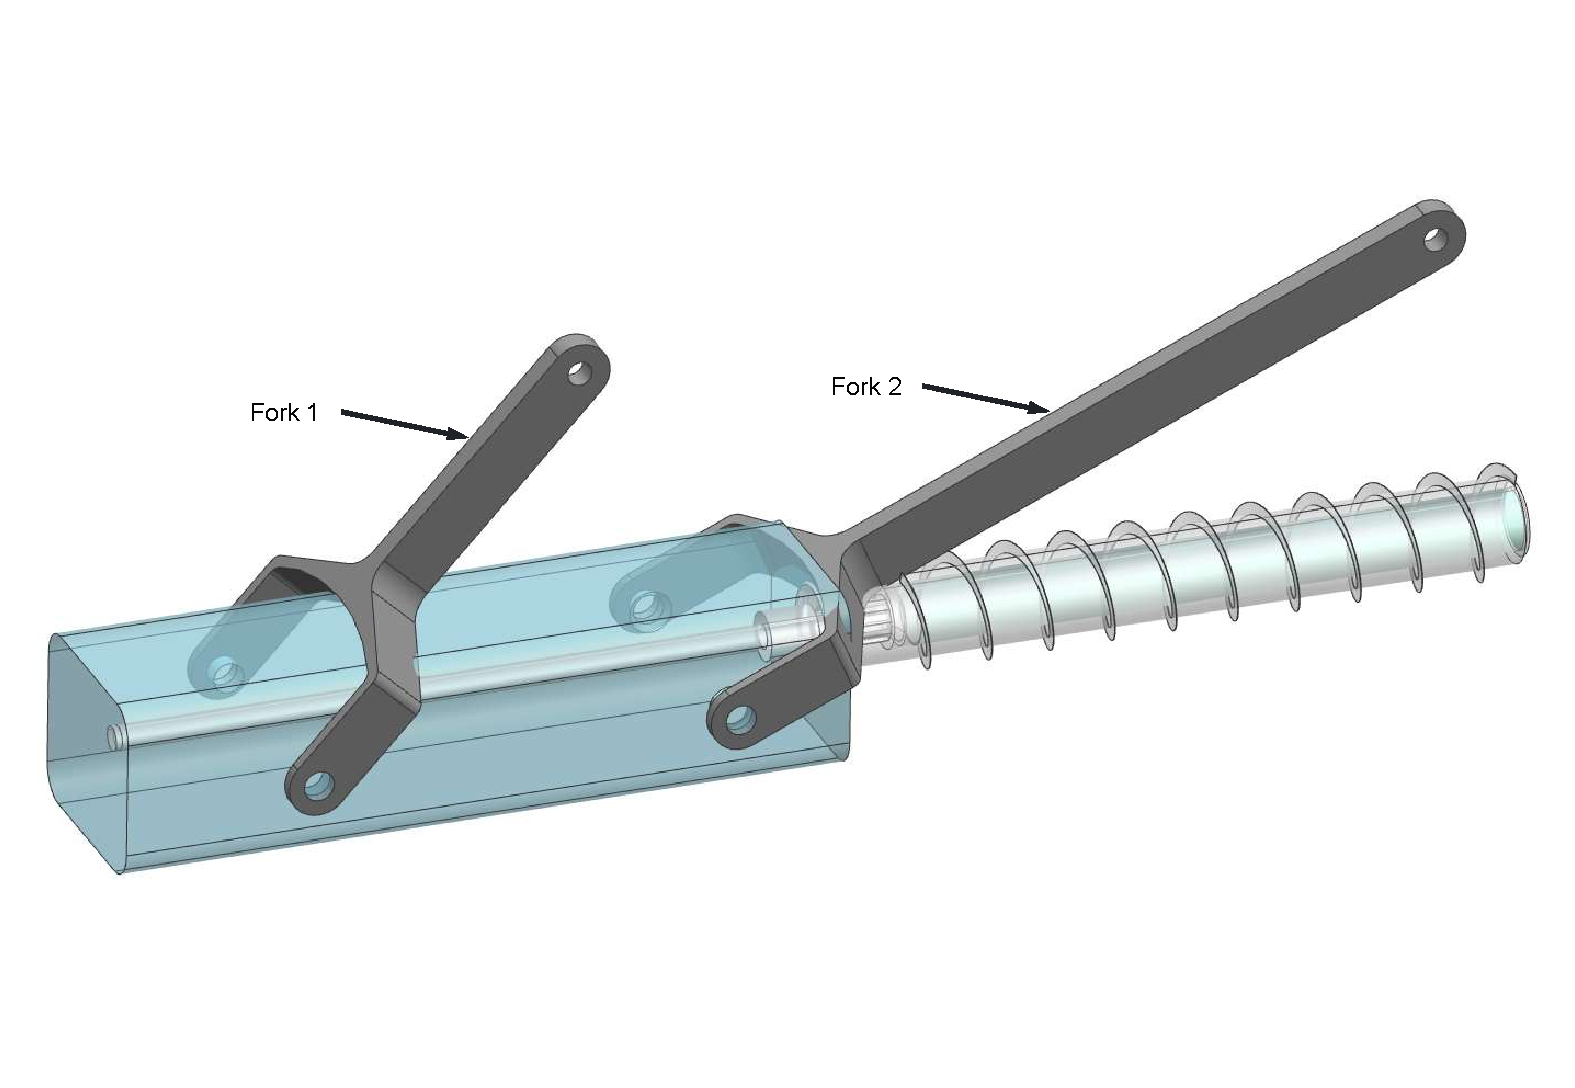
\includegraphics[width=0.55\textwidth]{Media/tcs_con_drill}}}}  \\[1em]
		& & & &  \\
		\multicolumn{2}{l}{$CON_{4}=CON_{F1}+CON_{F2} $} & & & \\[1em]
		\multicolumn{2}{l}{$CON_{4}= 1.56 \cdot 10^{-1}\ \frac{\W}{\K}$} & & & \\[4em]
		
		\hline
		Part &  Cross section & Length  & Material & Amount \\ \hline
		& & & & \\[-0.75em]
		Fork 1& $S_{F1}=40 \ \mm^2$ & $l_{F1}=90$ & Aluminium & 1 \\[0.5em]	
		Fork 1& $S_{F2}=40 \ \mm^2$ & $l_{F2}=150$ & Aluminium & 1 \\[5em]	
		
		
		\hline
		Name &  Linked Components &  \multicolumn{3}{c}{Geometry}\\ \hline
		& & & & \\[-0.5em]
		\textbf{Telescope} & \textbf{Camera} $\leftrightarrow$ \textbf{Chassis}  &  \multicolumn{3}{c}{\multirow{2}{*}{\adjustbox{valign=t}{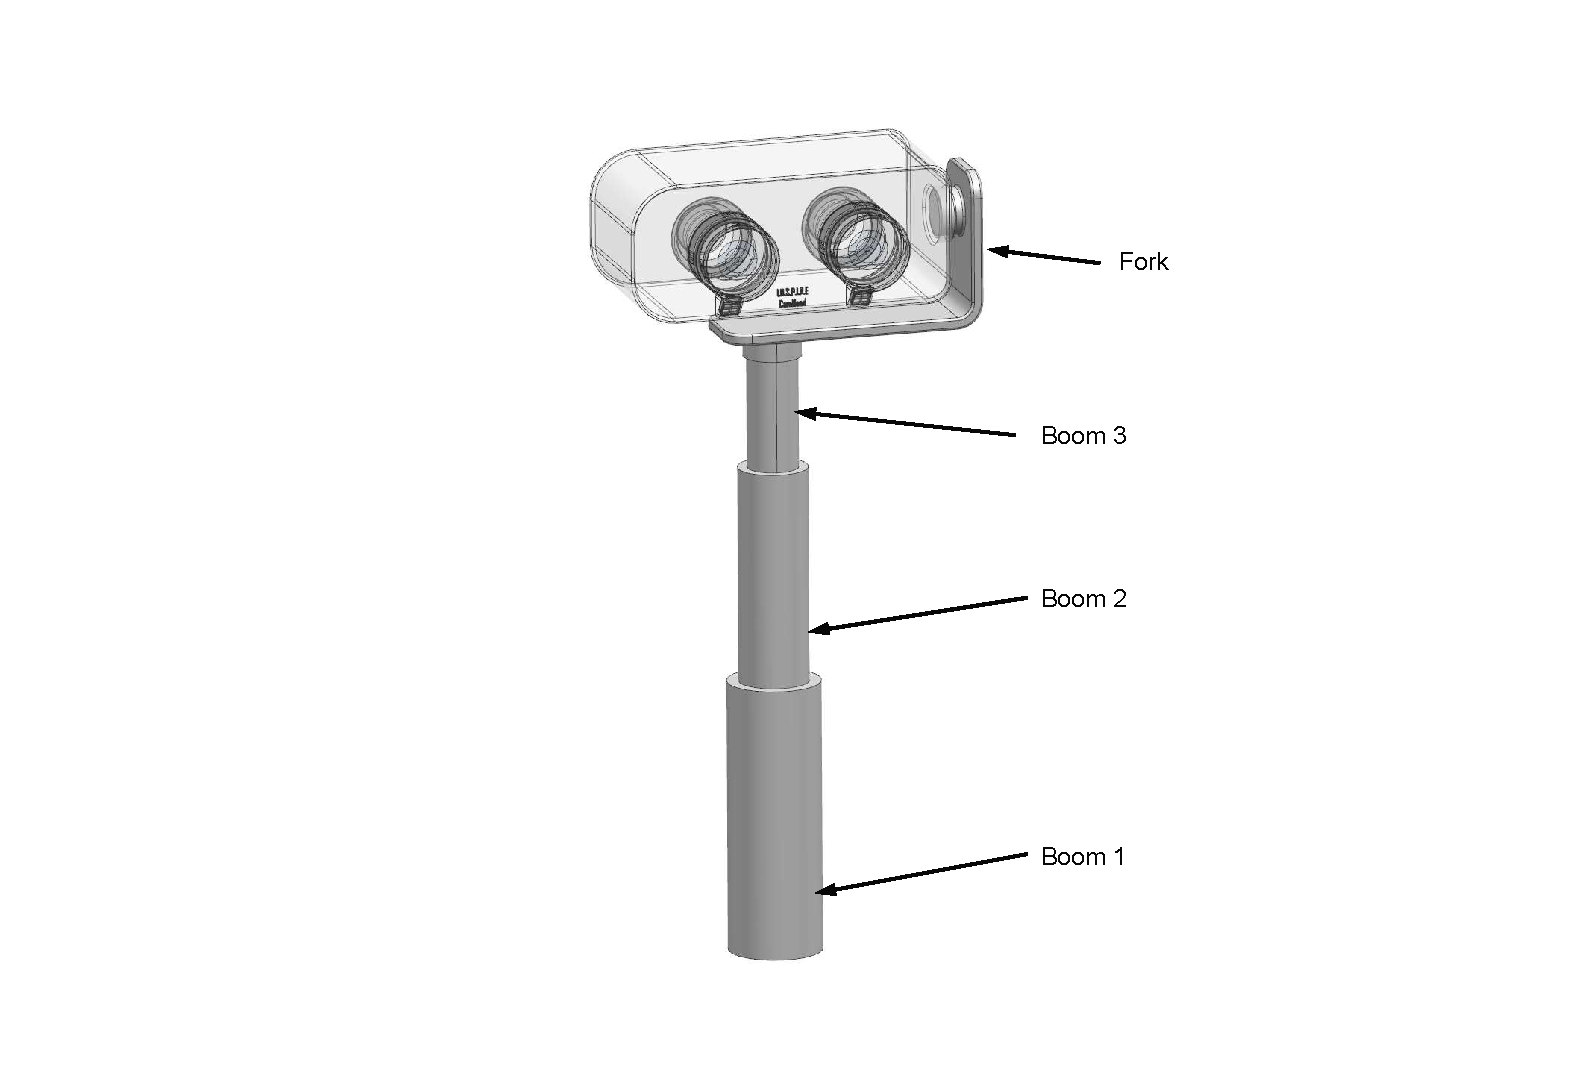
\includegraphics[width=0.25\textwidth]{Media/tcs_con_boom}}}}  \\[1em]
		& & & &  \\
		\multicolumn{2}{l}{$CON_6= \left( \frac{1}{CON_{B1}} +\frac{1}{CON_{B2}}+\frac{1}{CON_{B3}}+\frac{1}{CON_{F}} \right)^{-1} $} & & & \\[2em]
		\multicolumn{2}{l}{$CON_6= 7.81 \cdot 10^{-2}\ \frac{\W}{\K}$} & & &  \\[8em]
		\hline
		Part &  Cross section & Length  & Material & Amount \\ \hline
		& & & & \\[-0.75em]
		Boom 1 & $S_{B1}= 181 \ \mm^2$ & $l_{B1}=116 \ \mm$ & Aluminium & 1 \\[0.5em]
		Boom 2 & $S_{B2}= 134 \ \mm^2$ & $ll_{B2}=95 \ \mm$ & Aluminium & 1 \\[0.5em]
		Boom 3 & $S_{B3}= 97 \ \mm^2$ & $l_{B3}= 60\ \mm$ & Aluminium & 1 \\[0.5em]
		Fork & $S_{F}= 200\ \mm^2$ & $l_{F}=170\ \mm$ & Aluminium & 1 \\
		\label{tab:tcs_nodes2}
	\end{tabular}
\end{table}	

\begin{table}[htb]
\centering
\caption{Definition of heat conductance $CON=\frac{1}{R}$ between the nodes according to \autoref{fig:tcs_network}.}
\begin{tabular}{l@{\qquad}cccc}		
		\hline
		Name &  Linked Components &  \multicolumn{3}{c}{Geometry}\\ \hline
		& & & & \\[-0.5em]
		\textbf{Suspension} & \textbf{Chassis} $\leftrightarrow$ \textbf{Node$_1$}  &  \multicolumn{3}{c}{\multirow{2}{*}{\adjustbox{valign=t}{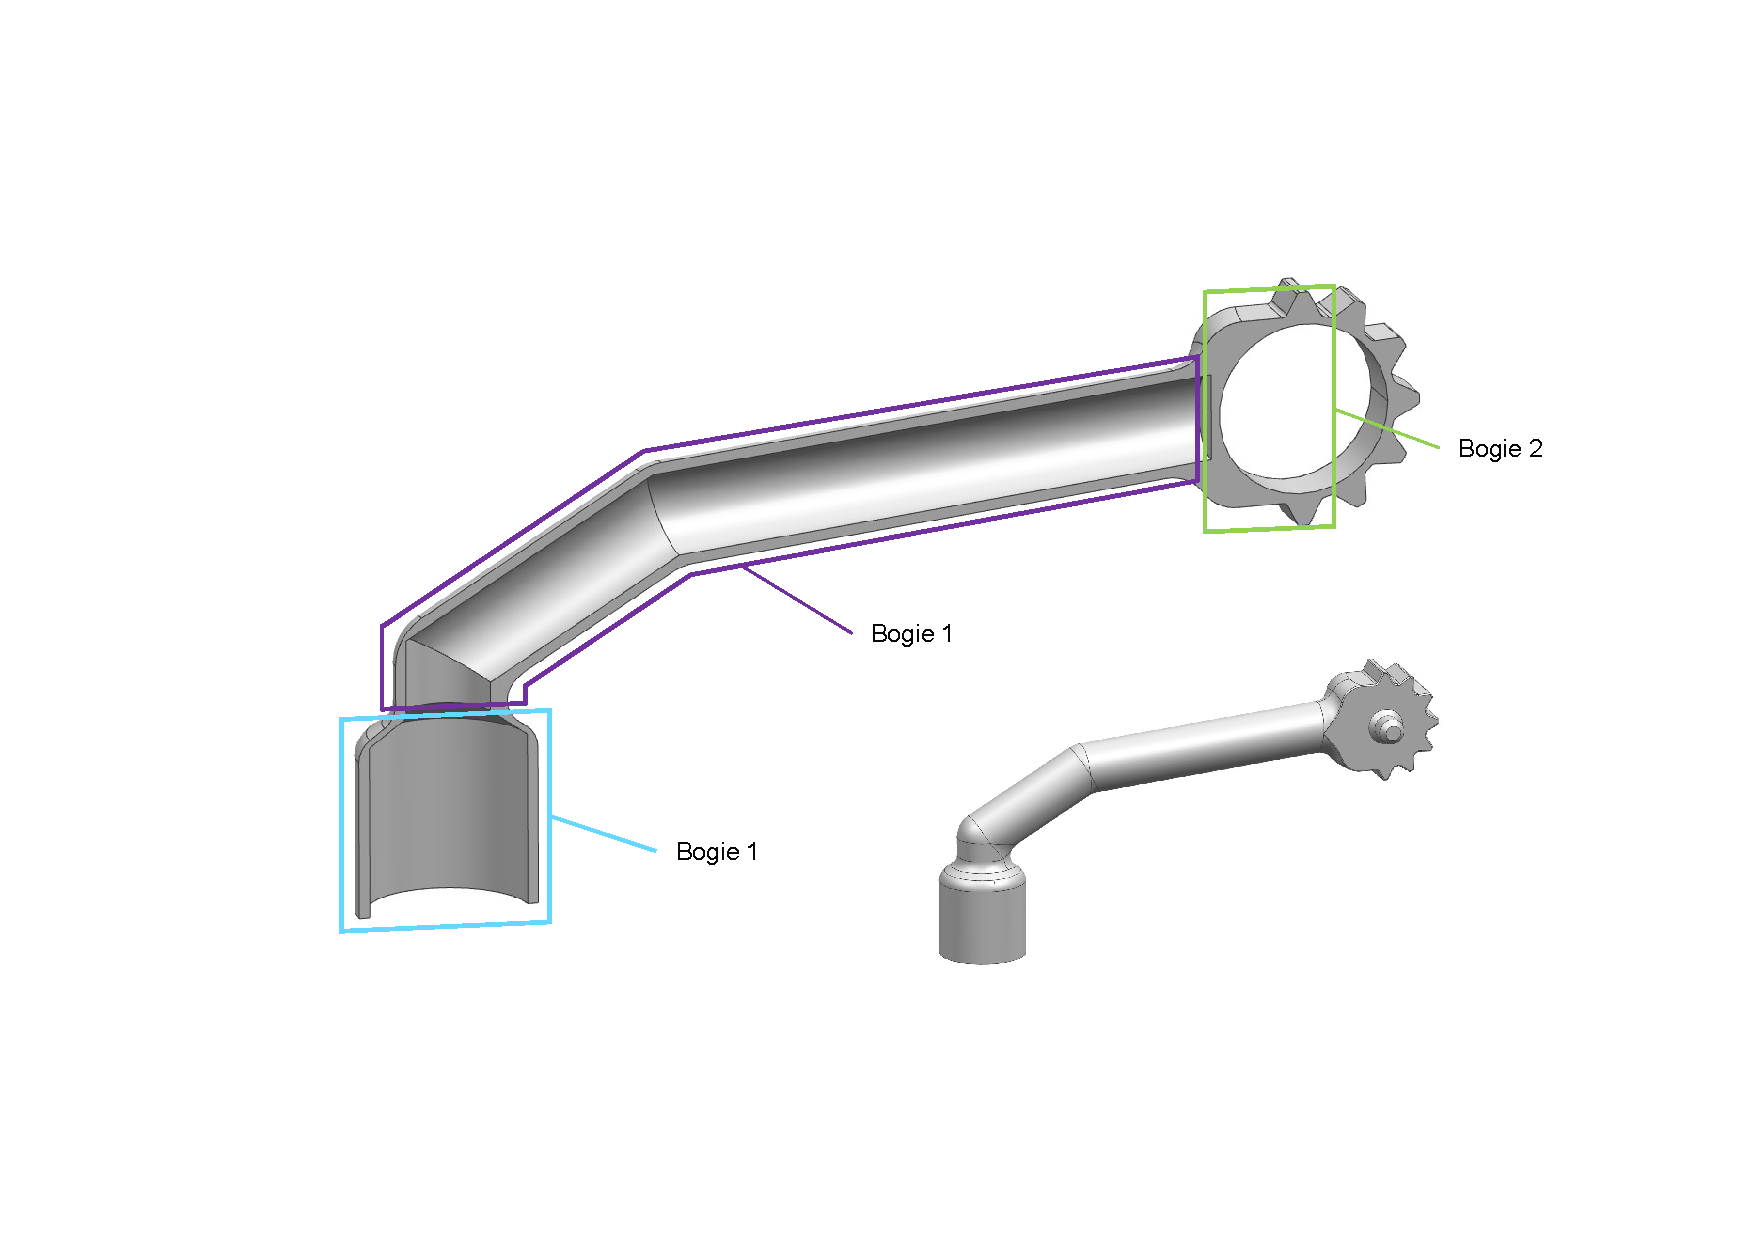
\includegraphics[width=0.455\textwidth]{Media/tcs_con_bogie}}}}  \\[1em]
		& & & &  \\
		\multicolumn{2}{l}{$CON_7=\left( \frac{1}{CON_{B1}} +\frac{1}{CON_{B2}}+\frac{1}{CON_{B3}}\right)^{-1}$} & & & \\[1em]
		\multicolumn{2}{l}{$CON_7= 1.30 \cdot 10^{-1}\ \frac{\W}{\K}$} & & & \\[6em]
		
		\hline
		Part &  Cross section & Length  & Material & Amount \\ \hline
		& & & & \\[-0.75em]
		Bogie 1 & $S_{B1}=275 \ \mm^2$ & $t_{B1}=20\ \mm$ & Aluminium & 1 \\[0.5em]
		Bogie 2 & $S_{B2}=113 \ \mm^2$ & $t_{B2}=162\ \mm$ & Aluminium & 1 \\[0.5em]
		Bogie 3 & $S_{B3}=201 \ \mm^2$ & $t_{B3}=37\ \mm$ & Aluminium & 1 \\[5em]		

		\hline
		Name &  Linked Components &  \multicolumn{3}{c}{Geometry}\\ \hline
		& & & & \\[-0.75em]
		\textbf{Mounting} & \textbf{Steer Engine} $\leftrightarrow$ \textbf{Node$_1$}  &  \multicolumn{3}{c}{\multirow{2}{*}{\adjustbox{valign=t}{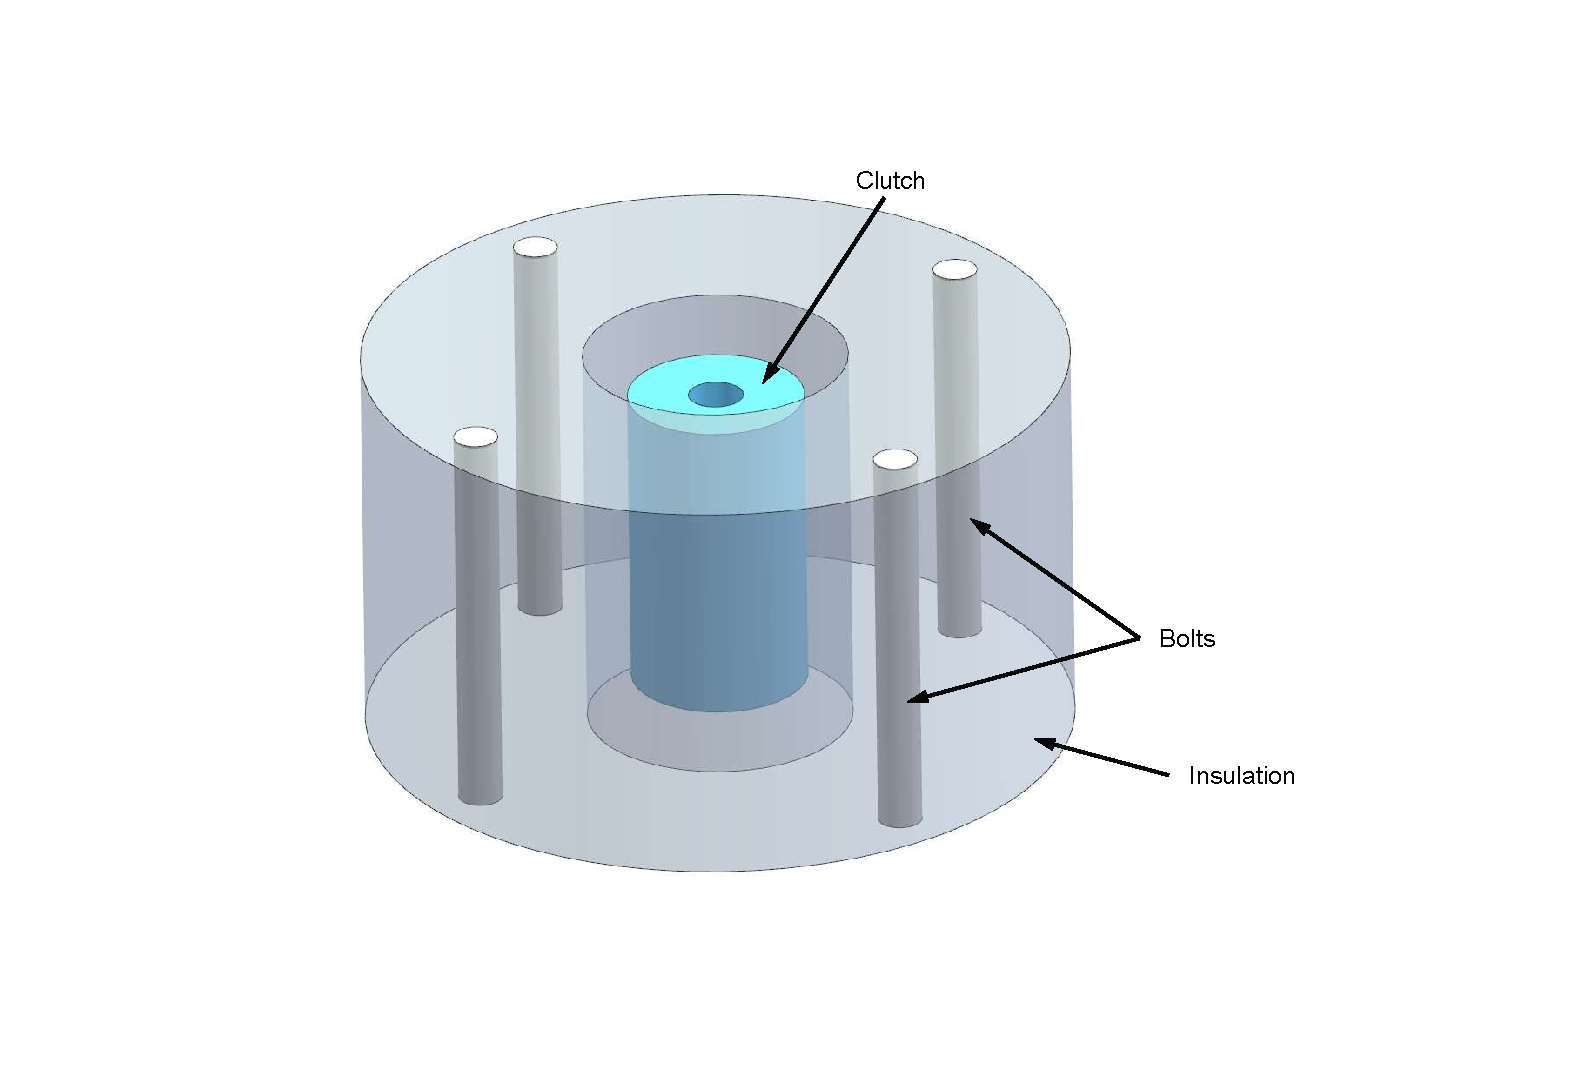
\includegraphics[width=0.4\textwidth]{Media/tcs_con_steer}}}}  \\[1em]
		& & & &  \\
		\multicolumn{2}{l}{$CON_8=CON_C+CON_I+n_B\cdot CON_B  $} & & & \\[2em]
		\multicolumn{2}{l}{$CON_8= 7.62\cdot 10^{-1}\ \frac{\W}{\K}$} & & &  \\[6em]
		\hline
		Part &  Cross section & Thickness  & Material & Amount \\ \hline
		& & & & \\[-0.75em]
		Clutch & $S_{C}= 45.4 \ \mm^2$ & $t_{C}=14 \ \mm$ & Aluminium  & 1 \\[0.5em]
		Insulation & $S_{I}= 691 \ \mm^2$ & $t_{I}=18 \ \mm$ & Aerogel & 1 \\[0.5em]
		Bolts & $S_{B}= 3.14 \ \mm^2$ & $t_{B}= 18\ \mm$ & Steel & 4 \\
		\hline
		\label{tab:tcs_nodes3}
	\end{tabular}
\end{table}	


\begin{table}[htb]
	\centering
	\caption{Definition of heat conductance $CON=\frac{1}{R}$ between the nodes according to \autoref{fig:tcs_network}.}
	\begin{tabular}{l@{\qquad}cccc}		
		Name &  Linked Components &  \multicolumn{3}{c}{Geometry}\\ \hline
		& & & & \\[-0.5em]
		\textbf{Wheel Fork} & \textbf{Node$_1$} $\leftrightarrow$ \textbf{Node$_2$}  &  \multicolumn{3}{c}{\multirow{2}{*}{\adjustbox{valign=t}{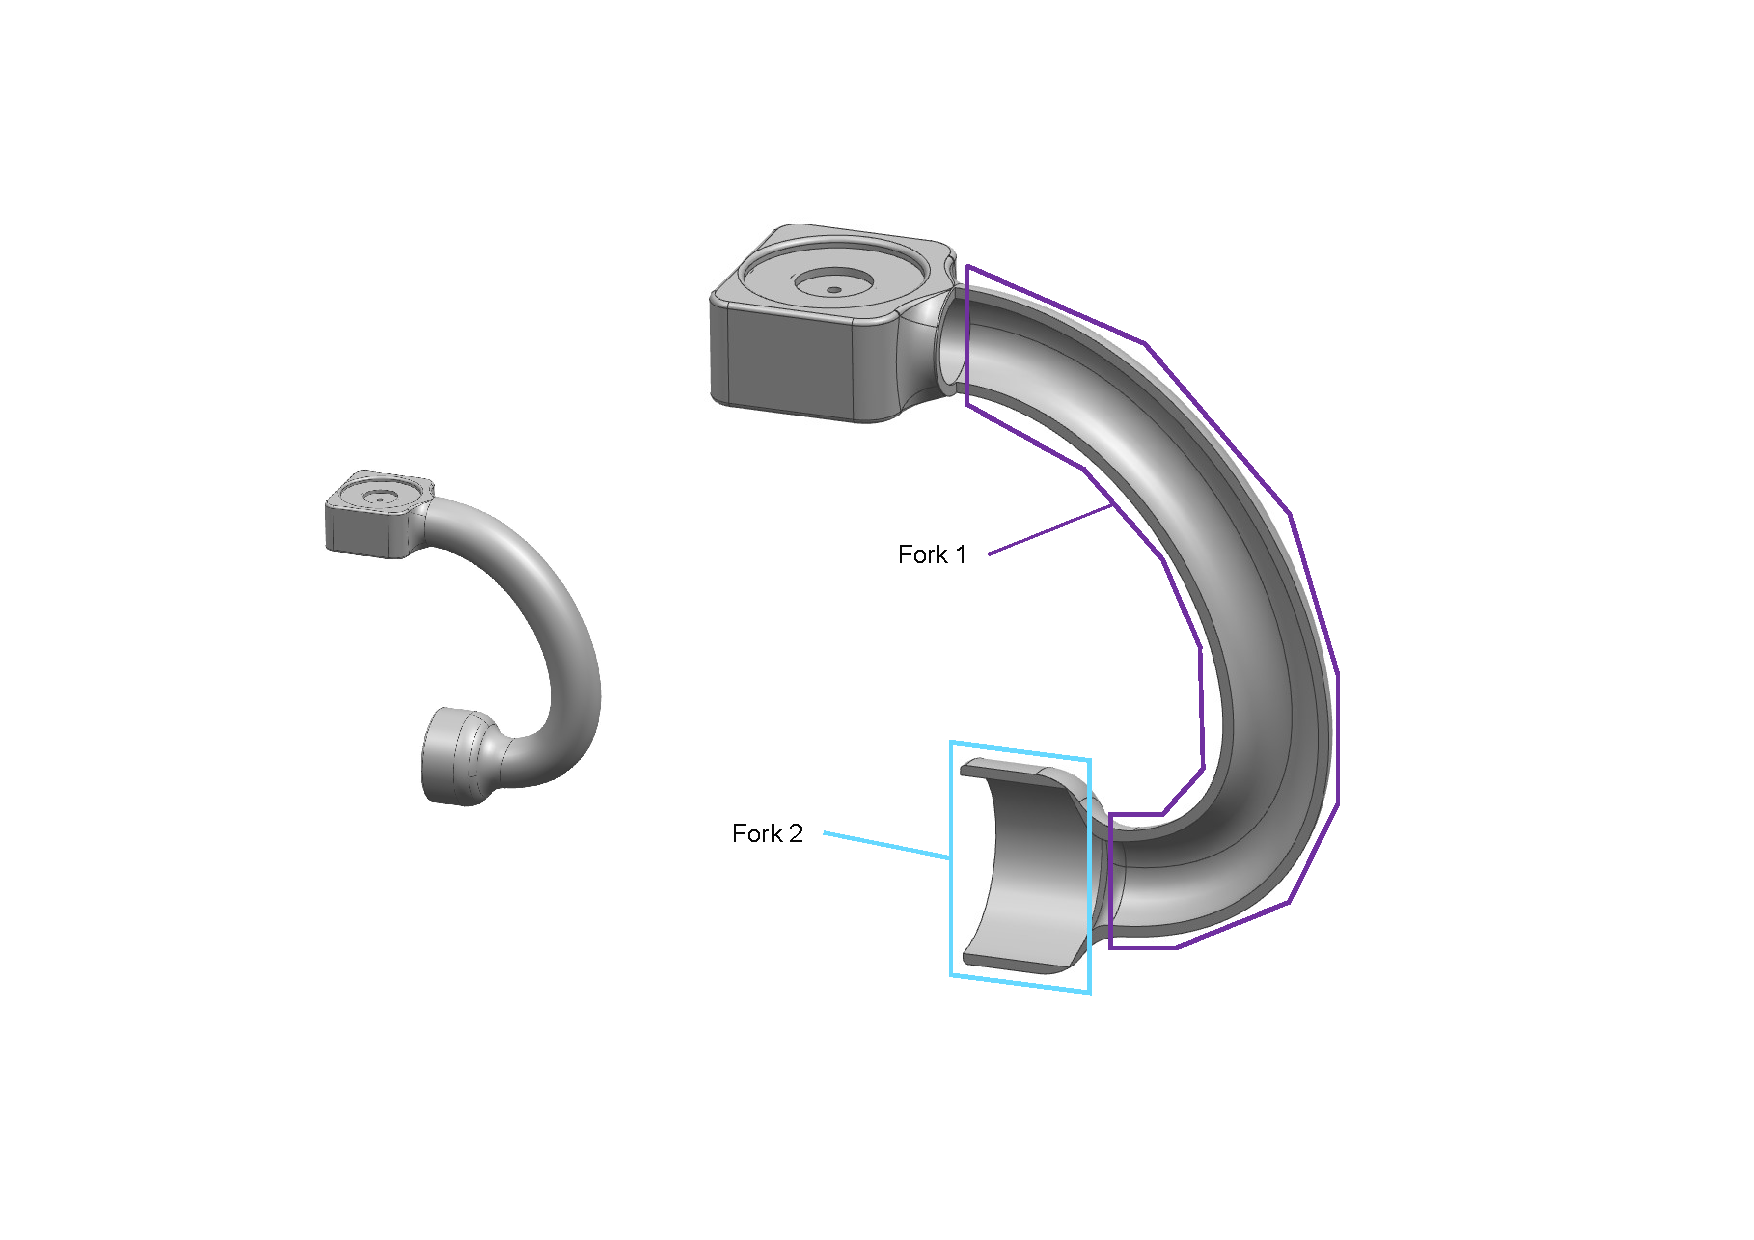
\includegraphics[width=0.45\textwidth]{Media/tcs_con_fork}}}}  \\[1em]
		& & & &  \\
		\multicolumn{2}{l}{$CON_{10}=\left( \frac{1}{CON_{F1}} +\frac{1}{CON_{F2}}\right)^{-1} $} & & & \\[1em]
		\multicolumn{2}{l}{$CON_{10}= 1.46 \cdot 10^{-1}\ \frac{\W}{\K}$} & & & \\[8em]
		
		\hline
		Part &  Cross section & Length  & Material & Amount \\ \hline
		& & & & \\[-0.75em]
		Fork 1& $S_{F1}=113 \ \mm^2$ & $l_{F1}=160$ & Aluminium & 1 \\[0.5em]	
		Fork 1& $S_{F2}=226 \ \mm^2$ & $l_{F2}=20$ & Aluminium & 1 \\[5em]	

		\hline
		Name &  Linked Components &  \multicolumn{3}{c}{Geometry}\\ \hline
		& & & & \\[-0.5em]
		\textbf{Mounting} & \textbf{Drive Engine} $\leftrightarrow$ \textbf{Node$_2$}  &  \multicolumn{3}{c}{\multirow{2}{*}{\adjustbox{valign=t}{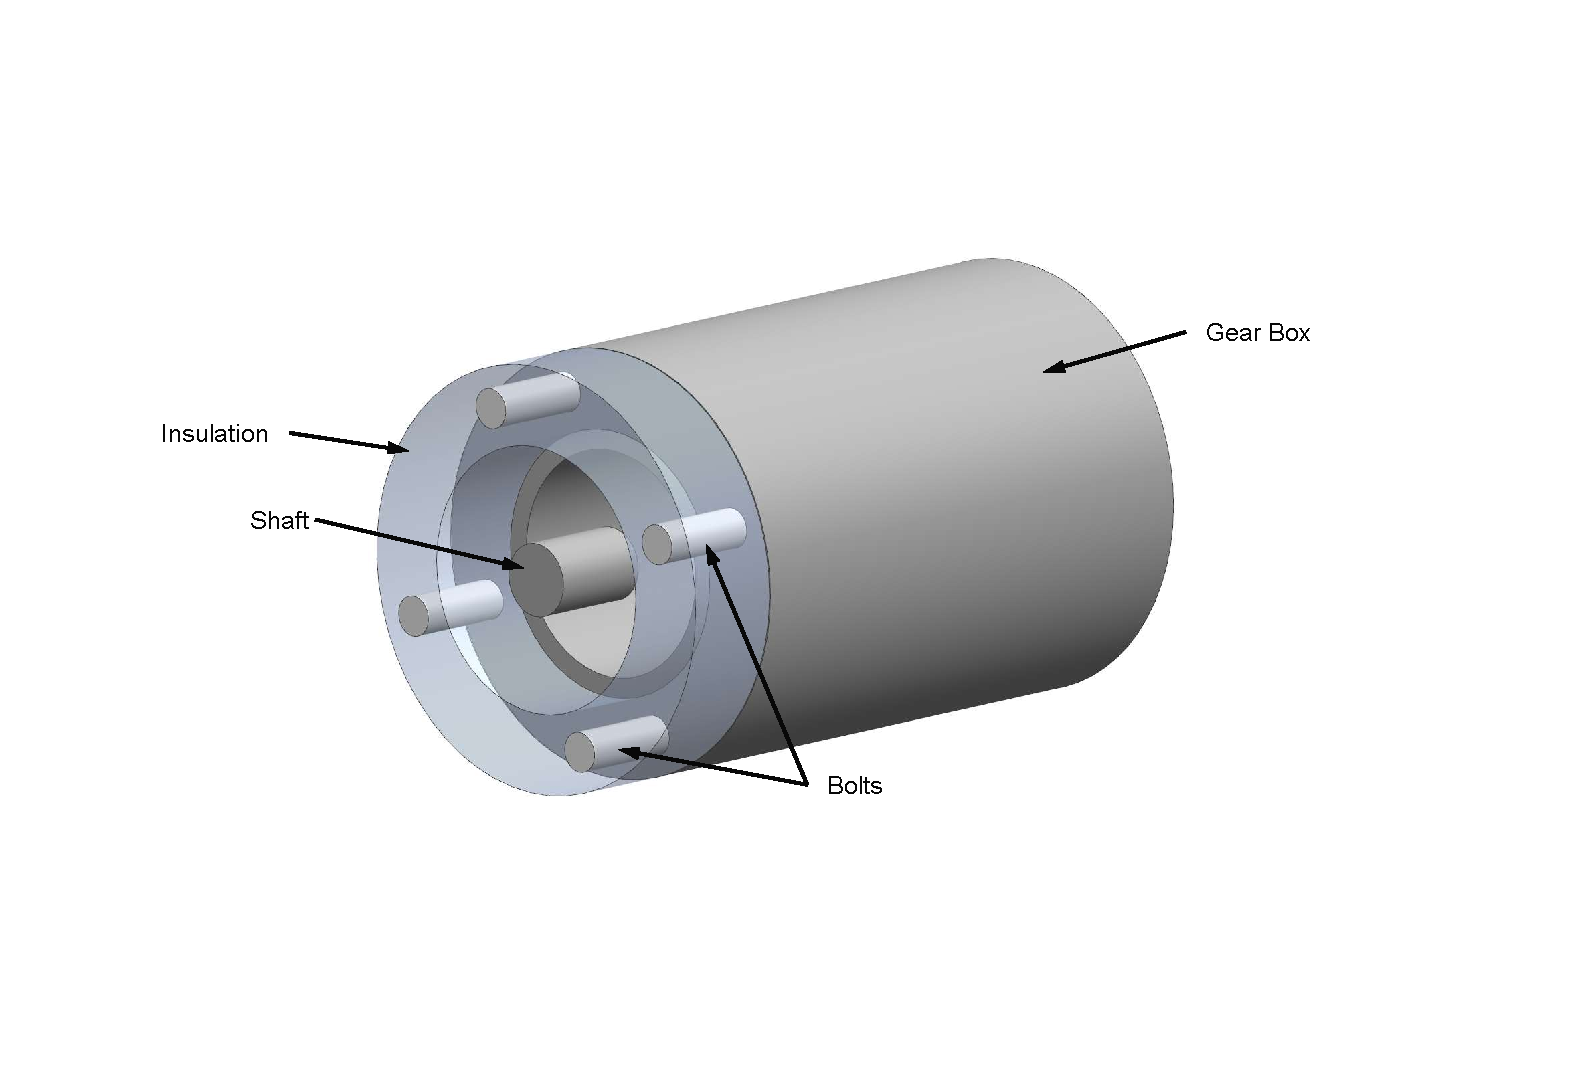
\includegraphics[width=0.5\textwidth]{Media/tcs_con_drive}}}}  \\[1em]
		& & & &  \\
		\multicolumn{2}{l}{$CON_{11}=  \left( \frac{1}{CON_G} +\frac{1}{CON_S+CON_I+n_B\cdot CON_B} \right)^{-1} $} & & & \\[2em]
		\multicolumn{2}{l}{$CON_{11}= 1.06 \cdot 10^{-1}\ \frac{\W}{\K}$} & & & \\[5em]
		
		\hline
		Part &  Cross section & Thickness  & Material & Amount \\ \hline
		& & & & \\[-0.75em]
		Gear Box & $S_{G}= 566 \ \mm^2$ & $t_{G}= 43.1\ \mm$ & Steel & 1 \\[0.5em]
		Shaft & $S_{S}= 23.8 \ \mm^2$ & $t_{S}=10 \ \mm$ & Steel & 1 \\[0.5em]
		Insulation & $S_{I}=490  \ \mm^2$ & $t_{I}=10 \ \mm$ & Aerogel  & 1 \\[0.5em]
		Bolts, M3 & $S_{B}=7.07  \ \mm^2$ & $t_{B}= 10\ \mm$ & Titan  & 4 \\[5em]	
	\end{tabular}
\label{tab:tcs_nodes4}
\end{table}	

\clearpage

\begin{table}[htb]
	\centering
	\caption{Definition of heat conductance $CON=\frac{1}{R}$ between the nodes according to \autoref{fig:tcs_network}.}
	\begin{tabular}{l@{\qquad}cccc}		
		\hline
		Name &  Linked Components &  \multicolumn{3}{c}{Geometry}\\ \hline
		& & & & \\[-0.5em]
		\textbf{Rim} & \textbf{Node$_2$} $\leftrightarrow$ \textbf{Ground}  &  \multicolumn{3}{c}{\multirow{2}{*}{\adjustbox{valign=t}{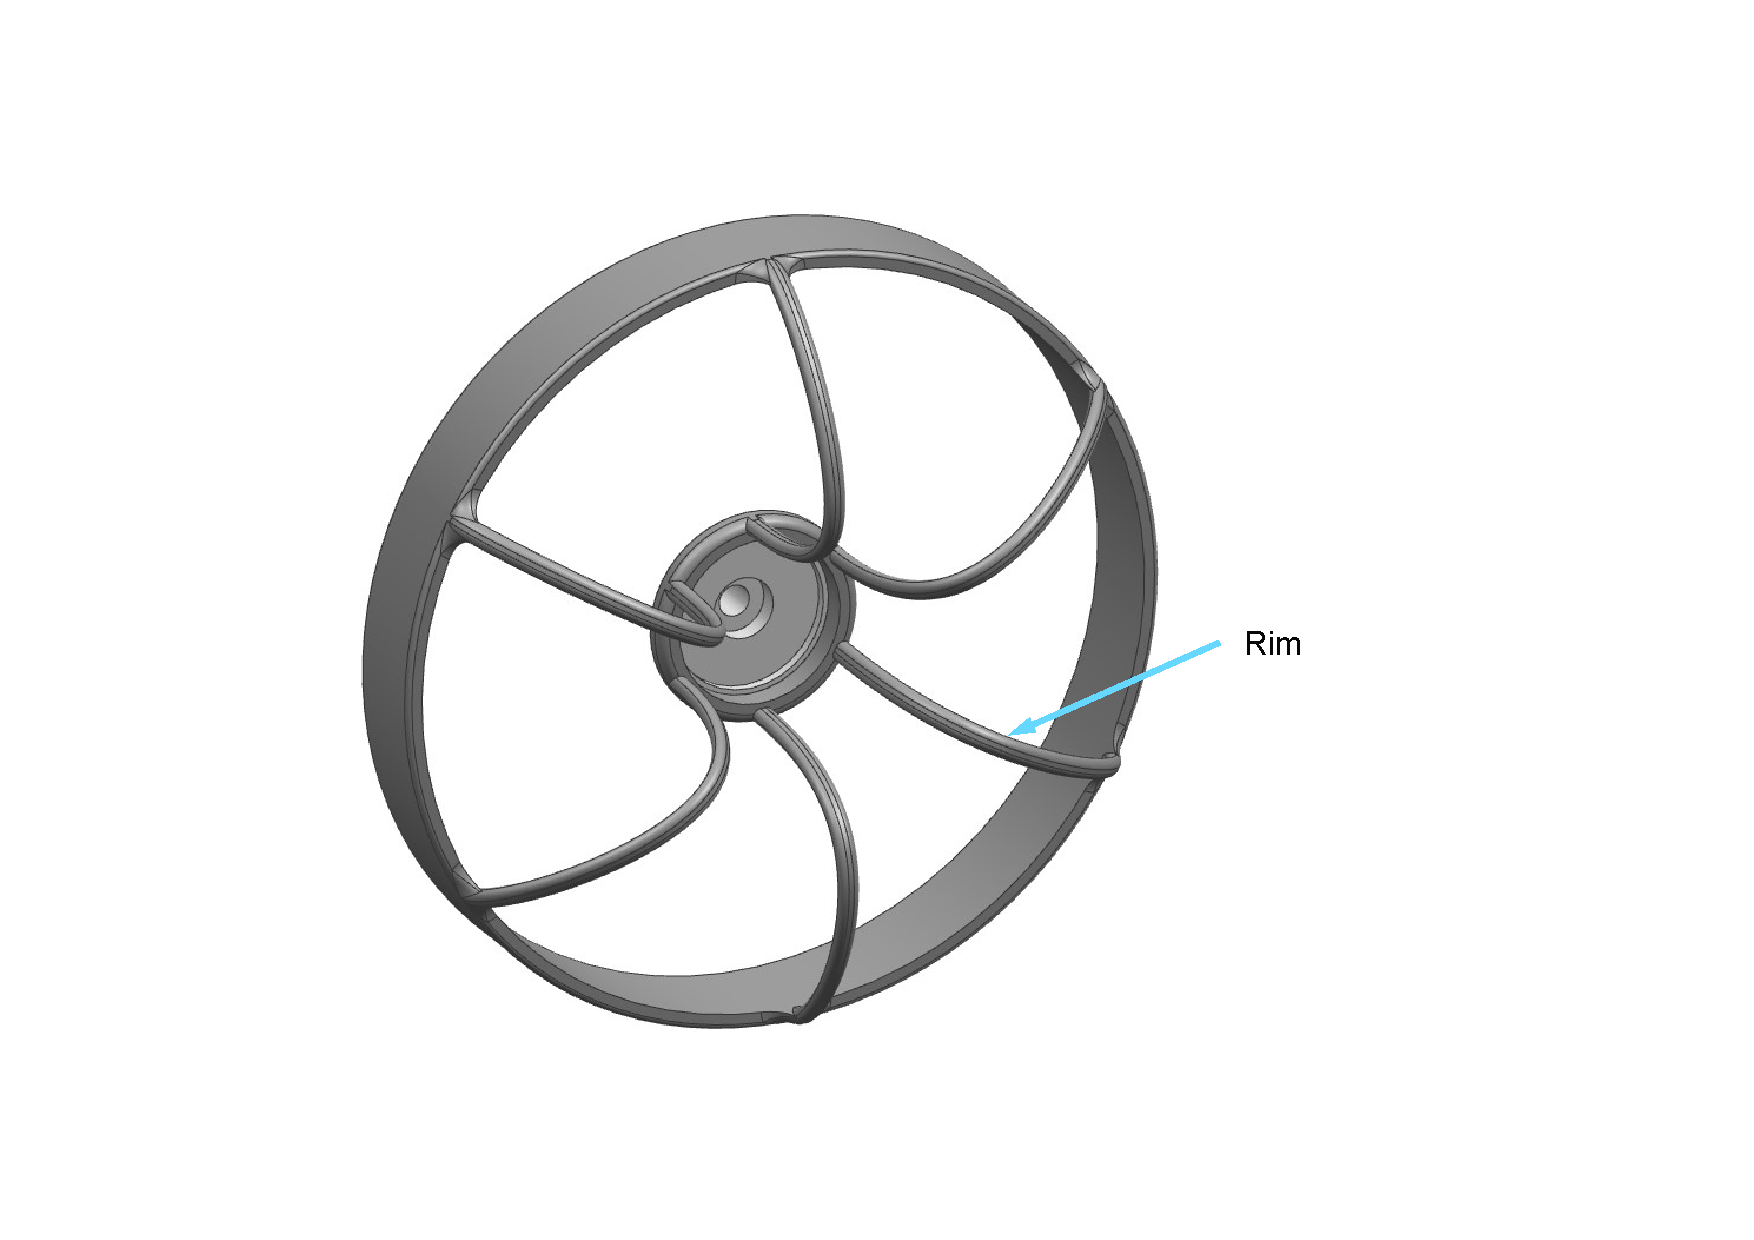
\includegraphics[width=0.3\textwidth]{Media/tcs_con_rim}}}}  \\[1em]
		& & & &  \\
		\multicolumn{2}{l}{$CON_{13}= 1.06 \cdot 10^{-1}\ \frac{\W}{\K}$} & & & \\[7em]
		
		\hline
		Part &  Cross section & Length  & Material & Amount \\ \hline
		& & & & \\[-0.75em]
		Rim & $S_R=8 \ \mm^2$ & $l_r=100\ \mm$ & Aluminium & 6 \\[1.5em]
		\multicolumn{5}{l}{\textit{Note}: It was assumed that the wheel temperature equals the surface temperature} \\
		\multicolumn{5}{l}{because of the thin rims and resulting low heat conduction.} \\
	\end{tabular}
\label{tab:tcs_nodes5}
\end{table}

\subsection{Heat switch} \label{sec:app_therm_3}

The characteristic of the switch conductance depends on the mean temperature $T_M$, shown by measurements in cite .
As this temperature won´t be calculated in the analysis, the corresponding component temperature $T_C$ shall be used.
In order to describe the characteristic, it was divided in three sections, \autoref{fig:tcs_switch03}.
The temperature where the disk decouples is $T_{toggle}=108 K$ and not applicable for the current application.
By reducing the height, the toggle temperature can be increased and the characteristic can be shifted to higher temperatures ("to the right").
It was assumed that the gradients of section 2 and 3 as well as the temperature range of section 2 keep constant.
The axis interception is a function the toggle temperature ($a_2=f(\Delta T_{toggle}),\ \Delta T_{Toggle}=T_{new}-T_{old}|_{toggle}$).
The used toggle temperature are listed in autoref

\begin{table}[H]
	\centering
	\caption{Toggle temperature and amount of bi-metallic heat switch.}
	\begin{tabular}{c@{\quad}ccc}
		\toprule
		Heat switch name  & Linked Components & Temperature  & Amount \\ \midrule
		$CON_{S1}$ & {Camera} $\leftrightarrow$ {Radiator} & -28\ $^\circ$C  & $n_{S1}=$4  \\[1em]
		$CON_{S2}$ & {EBay} $\leftrightarrow$ {Chassis} & -5\ $^\circ$C  & $n_{S2}=$2  \\[1em]
		$CON_{S3}$ & {Drive Engine} $\leftrightarrow$ {Node$_2$} & -20\ $^\circ$C  & $n_{S3}=1$  \\
		&											&						& (in total 4)  \\ \bottomrule
	\end{tabular}
	\label{tab:tcs_toggle}
\end{table}


\begin{table}[H]
	\centering
	\caption{Sections and range of the switch characteristic.}
	\begin{tabular}{c@{\qquad}rcl@{\qquad}l}
		\toprule
		Section & \multicolumn{3}{l}{Temperature range} & Heat conductance $CON_S= \frac{1}{R_t}$ \\ \midrule
		& & & &  \\[-0.5em]
		1 & $T_{toggle} >$ & $ T_C  $ & & $CON_{S}= 16.4 \cdot 10^{-3}\ \frac{\W}{\m^2 \K} = const.$\\[1.5em]
		2 & $T_{toggle}\leq$ & $ T_C $ & $ < T_1$ & $CON_{S} (T_C) = a_{1.1} \cdot T_C+ a_{1.2}$\\[1em]
		& & & & $a_{1.1}= +1.272\cdot 10^{-3}\ \frac{\W}{\m^2 \K^2}$ \\[1em]
		& & & & $  a_{1.2}= -1.272\cdot 10^{-3}\ \frac{\W}{\m^2 \K^2}\cdot \Delta T_{Toggle}-0.117\ \frac{\W}{\m^2 \K}$  \\[2em]
		3 & & 	$ T_C$ & $^ > T_1$ & $CON_{S}(T_C) = a_{2.1} \cdot T_C+ a_{2.2}$\\[1em]
		& & & & $a_{2.1}=+ 333\cdot 10^{-6}\ \frac{\W}{\m^2 \K^2}$ \\[1em]
		& & & & $  a_{2.2}= -333\cdot 10^{-6}\ \frac{\W}{\m^2 \K^2}\cdot \Delta T_{Toggle}-28.3 \cdot 10^{-3}\ \frac{\W}{\m^2 \K}$  \\[1em] \bottomrule
	\end{tabular}
	\label{tab:tcs_section}
\end{table}

\begin{figure}[htb]
	\centering
	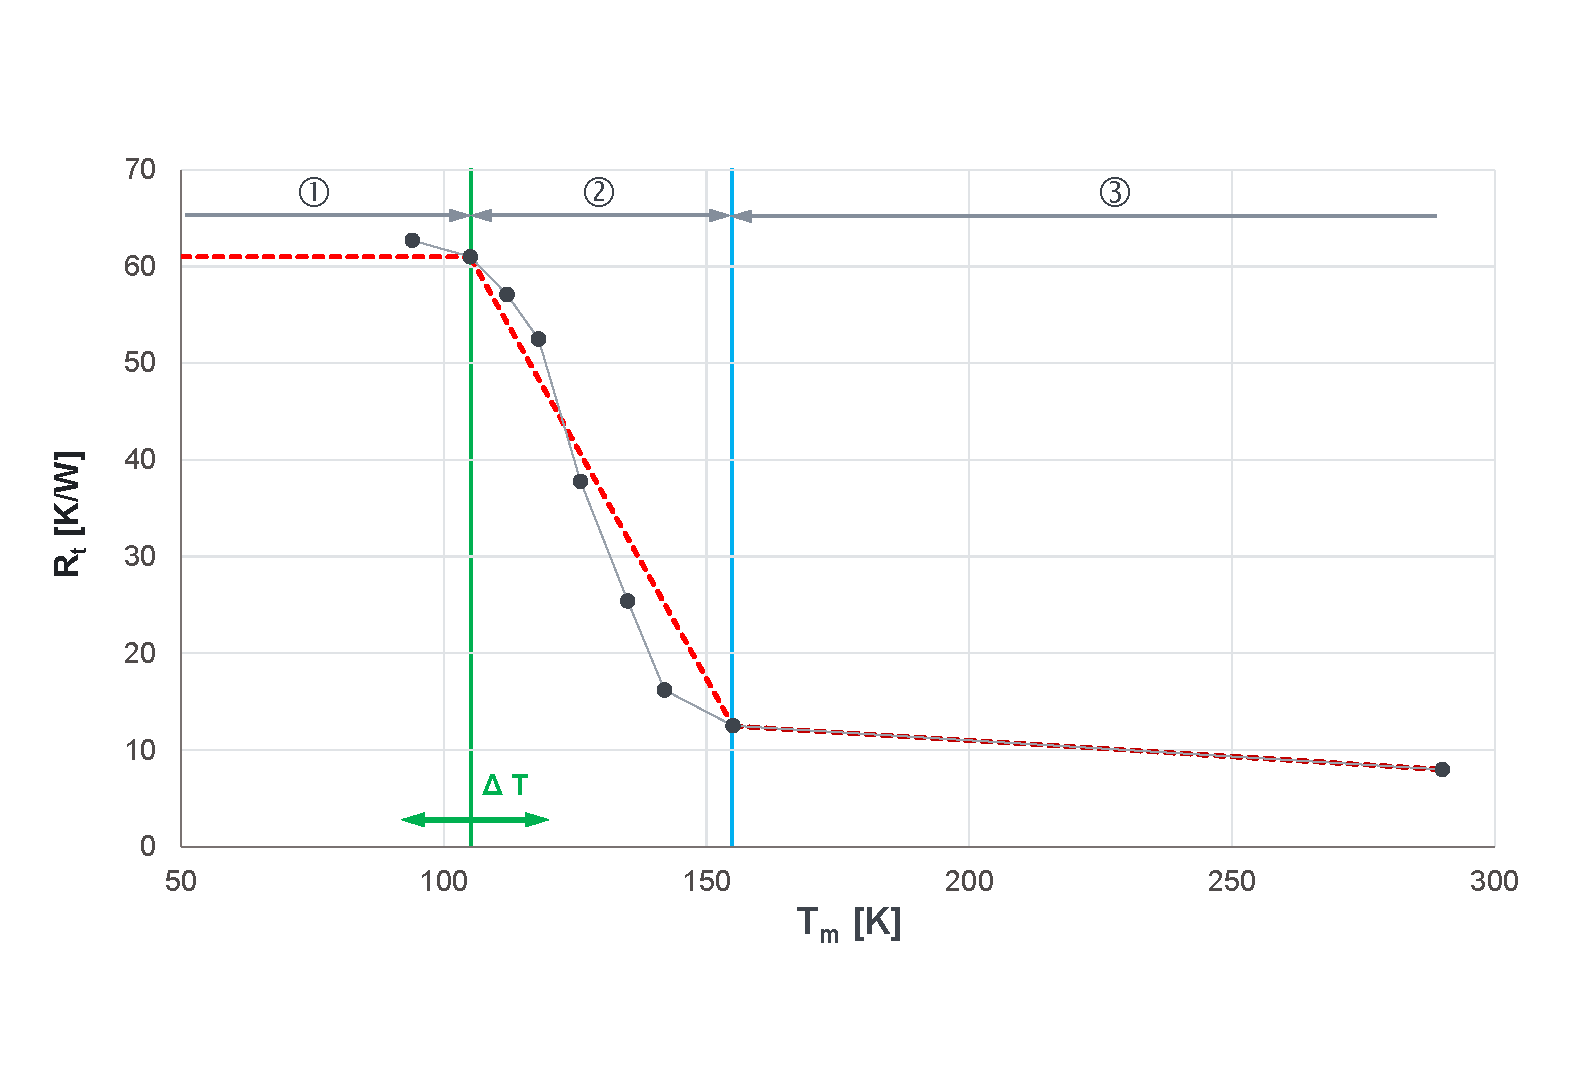
\includegraphics[width=1\textwidth]{Media/tcs_diag_section}
	\caption{Conductance characteristic of heat switch diveded in sections.}
	\label{fig:tcs_switch03}
\end{figure}

\subsection{Rover absorptivity} \label{sec:app_therm_4}
The rover position relative to the direct sun radiation is given by the ecliptic longitude $\lambda_R$ and latitude $\delta_R$ angle, where the axis $x_E$ points always to the sun, \autoref{fig:tcs_rad2}.
The amount of solar radiation $S_0$ absorbed by the rover surfaces depends on the sun altitude and can be determined by the view factor $\varphi$, see \autoref{fig:tcs_rad1}.
The view factors during the eclipse are set to zero.

\begin{table}[H]
	\begin{tabular}{l@{\qquad}ll}
		View Factor 1,& horizontal surface:& $ \varphi_1=\cos (\lambda_R) \cdot \cos (\delta_R)  $ \\
		View Factor 2, & vertical surface: &$ \varphi_2=\cos (90^{\circ}-\lambda_R) \cdot \cos (\delta_R)  $\\
	\end{tabular}
\end{table}

\begin{figure}[h]
	\centering
	\subfloat[View factor depending on the absorption surface.]{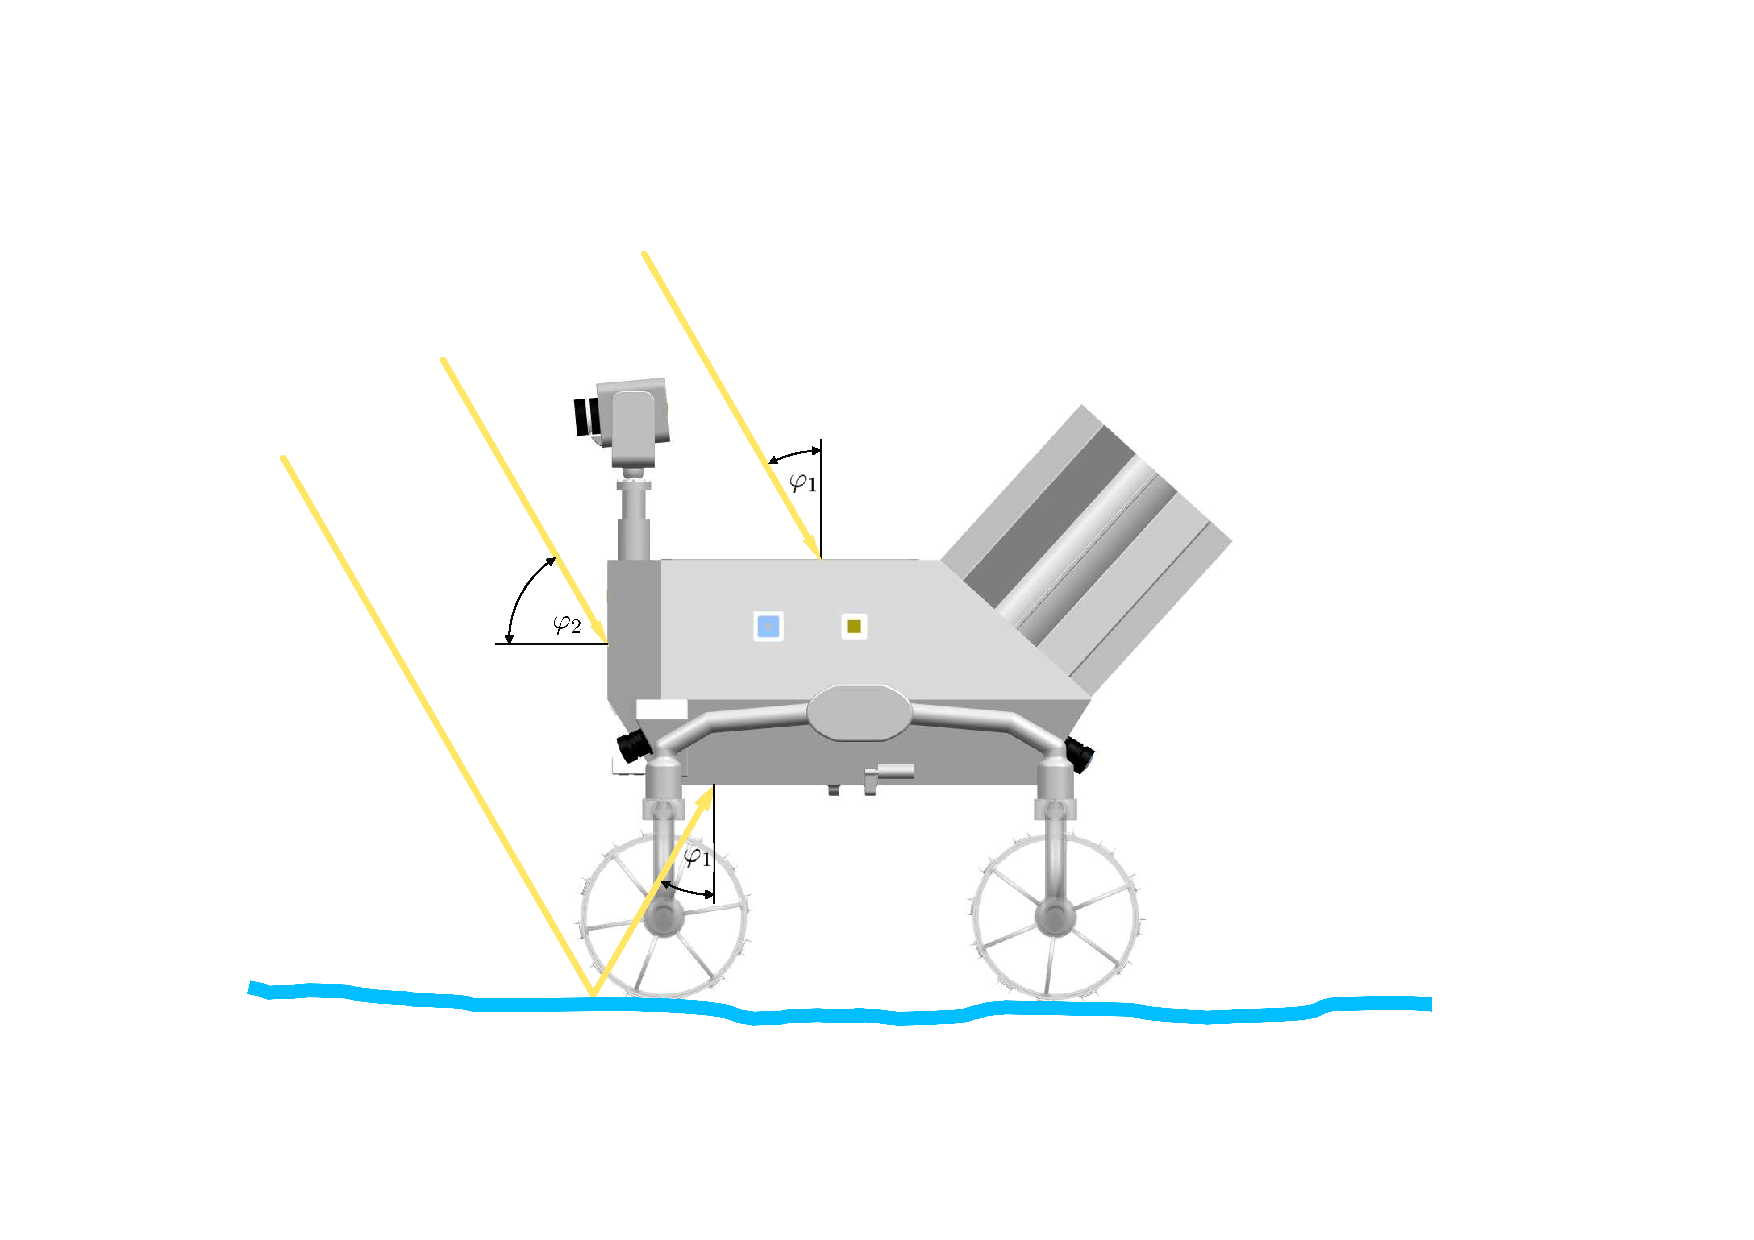
\includegraphics[height=0.4\textwidth]{Media/tcs_rover_rad}\label{fig:tcs_rad1}}\qquad\qquad
	\subfloat[Definition of ecliptic longitude $\lambda_R$ and latitude $\delta_R$ of the rover on Europa.]{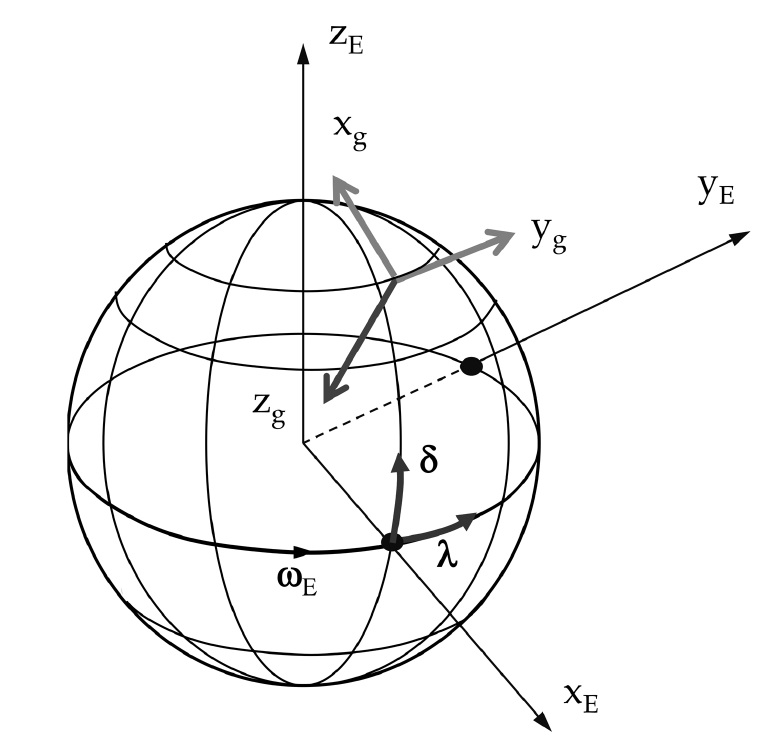
\includegraphics[height=0.3\textwidth]{Media/tcs_angle.png}\label{fig:tcs_rad2}}
	\caption{Bi-metallic heat switch, \cite{ref_tcs_04}.}
	\label{fig:tcs_rad}
\end{figure}


\subsection{Input Values} \label{sec:app_therm_5}
\begin{table}[H]
	\centering
	\caption{Temperatur limits of the rover components.}
	\begin{tabular}{l@{\qquad\qquad}cc}
		\toprule 
		& \multicolumn{2}{l}{Temperature limits in [$^\circ$C]} \\ 
		Component	&	min. & max. \\ \midrule
		OBC & -55 & 70 \\
		Transmitter & -10 & 50 \\
		Receiver & -30 & 70  \\
		PCDU & -40 & 60  \\
		Battery & -20 & 60 \\
		Camera & -40 & 70  \\
		Objektive  & -40 & 71  \\
		Steering Engine & -30 & 100 \\
		Drive Engine & -40 & 100 \\
		Drive Gear & -40 & 100  \\ \bottomrule
	\end{tabular}
	\label{tab:tcs_limits}
\end{table}

\begin{figure}[H] 
	\centering
	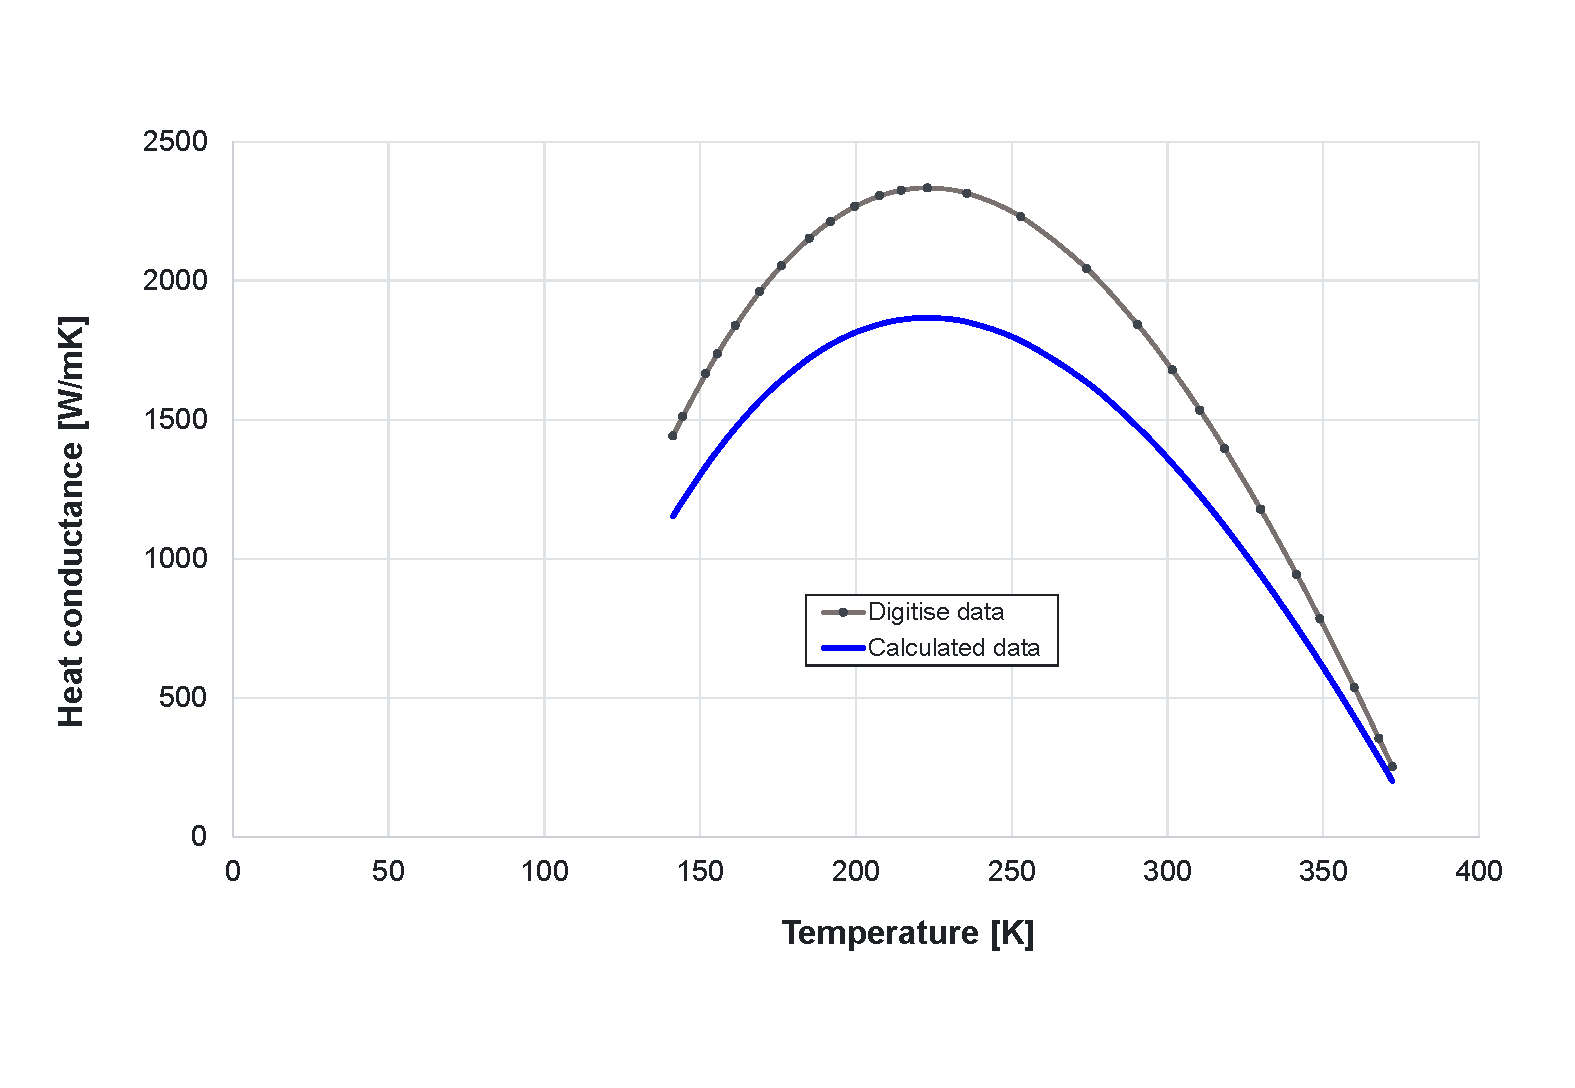
\includegraphics[width=0.8\textwidth]{Media/tcs_lynx_calc}
	\caption{Digitalised \cite{ref_tcs_01} and calculated heat conduction in comparison.}
	\label{fig:tcs_lynx}
\end{figure}
The characteristic of the \textit{LyNX}\textsuperscript{\tiny\textregistered} conduction was approximated with following function,
\begin{equation}
\lambda(T)= \left(1.76 \cdot 10^{-4}\ \frac{\W}{\m \K^4} \cdot T^3 -2.37\cdot 10^{-1}\ \frac{\W}{\m \K^3} \cdot T^2 +79.5 \frac{\W}{\m \K^2} \cdot T -5.55\cdot 10^{3}\ \frac{\W}{\m \K}\right) \cdot f_{r}  
\label{eq:tcs_lynx}
\end{equation}
with the reduction factor $f_{r}$=0.8.

\begin{table}[H]
	\centering
	\caption{Dimensions of the thermal straps \textit{LyNX}\textsuperscript{\tiny\textregistered}.}
	\begin{tabular}{l@{\quad}cc}
		\toprule
		Linked Components & Cross section  & Length$^{1)}$  \\ \midrule
		EBay $\leftrightarrow$ RTG & 42\ mm$^2$ & 230 mm  \\[0.25em] 
		Drill $\leftrightarrow$ RTG &10 \ mm$^2$ &345 \ mm \\[0.25em] 
		Steer Engine $\leftrightarrow$ RTG & 36\ mm$^2$&644\ mm  \\[0.25em] 
		Drive Engine $\leftrightarrow$ RTG &42 \ mm$^2$&897\ mm  \\[0.25em] \bottomrule
		& &   \\[-0.5em]
		\multicolumn{3}{l}{$^{1)}$\ Du to uncertainties the length was increased about 15\%.}\\[1em]
	\end{tabular}
	\label{tab:tcs_lynx}
\end{table}

The Europa surface temperature varies at the  equator between $T_{e,min}=80~\K$ and\\ $T_{e,max}=130~\K$, depending on the sun inclination.
The temperature at the pole is ${T_{Pole}=50~\K}$, \cite{Europa}.
It was assumed that the surface temperature depends on the sun altitude.
A trigonometrical interpolation was defined as follows.
\[ T_{Surface}(\lambda, \delta) = T_{Pole} + \cos (\delta) \cdot [(T_{e,min}+\cos (\lambda)\cdot (T_{e,max}-T_{e,min}))-T_{Pole}] \]
For $\lambda$ and $\delta$ see \autoref{sec:app_therm_4}.\\

\begin{table}[H]
	\centering
	\caption{Minimum and maximum of surface emissivity and absorptivity values, \cite{ref_tcs_05}.}
	\begin{tabular}{l@{\qquad\qquad}cc@{\qquad\qquad}cc}
		\toprule
		& \multicolumn{2}{l}{Emissivity [-]} & \multicolumn{2}{l}{Absorptivity [-]}  \\ 
		Surface finishing	&	min. & max. 	&	min. & max.   \\\midrule
		Aluminium, polished & &0.05  & & 0.2   \\
		Aluminium, sand blasted & &0.2  & & 0.4   \\
		White paint & 0.8 & 0.9 & 0.2 & 0.5  \\ \bottomrule
		& & & & \\
	\end{tabular}
	\label{tab:tcs_surface}
\end{table}


\begin{table}[H]
	\centering
	\caption{Heat conductivity in $\frac{\W}{\m \K}$}
	\begin{tabular}{l@{\qquad\qquad}c@{\qquad\qquad}c@{\qquad\qquad}l}
		\toprule
		Material & Nominal & Used & Source \\ \midrule
		Aerogel & 0.002 - 0.05 & 0.05 & \cite{ref_tcs_03} \\
		Aluminium$^{1)}$  & 110 - 220 & 220 & \cite{ref_tcs_10}, \cite{ref_tcs_11}, \cite{ref_tcs_12} \\
		Steel$^{1)}$ & 15 - 43 & 45 & \cite{ref_tcs_08}, \cite{ref_tcs_09} \\ 
		Titan  & 7.1  & 7.1 & \cite{ref_tcs_06}, \cite{ref_tcs_07} \\\bottomrule
		&&&\\[-0.75em]
		\multicolumn{4}{l}{\small{$^{1)}$\  Depends on the alloying component, a conservative value was choosen.}}\\
	\end{tabular}
	\label{tab:tcs_conduct2}
\end{table}

\begin{table}[H]
	\centering
	\caption{Radiation surface and finishing of components.}
	\begin{tabular}{l@{\qquad}l@{\qquad}ll}
		\toprule
		Part  & Surface [$\m^2$] & Finishing & Note \\ \midrule
		Chassis - top/bottom & $S_{Ch1}=0.086$ &  white paint & for albedo\\
		Chassis - side & $S_{Ch2}=0.081$ &  white paint & for albedo\\
		Chassis - total & $S_{Ch3}=0.423$ &  white paint & for emissivity\\
		RTG& $S_{RTG}=0.086$ & white paint & konstant emissivity of 0.9\\
		Electric Bay& $S_{Bay}=0.146$ & AL, sand blastet & \\
		Camera - housing & $S_{Cam}=0.027$ & AL, sand blastet &\\
		Camera - radiator & $S_{Rad}=0.066$ & white paint &  \\
		Steer Engine& $S_{E,S}=0.002$ & white paint& \\
		Drive Engine& $S_{E,D}=0.003$ &white paint & \\
		Bogie & $S_{B}=0.018$ &white paint & \\
		Wheel Fork& $S_{F}=0.008$ &white paint & \\ \bottomrule
		&&& \\
		\multicolumn{3}{l}{The cross sections were taken form the CAD model.}
	\end{tabular}
	\label{tab:tcs_surf}
\end{table}

\clearpage

\setcounter{figure}{0}
\setcounter{table}{0}

\section{Radiation}

\label{sec:AppendixRadiation}

In this chapter, detailed calculations are performed on which \autoref{sec:Radiation} is based on. All calculations and figures in \autoref{sec:AppendixRadiation} are performed with SPENVIS unless otherwise stated. In order to simulate the radiation on Europa an orbit around Jupiter is simulated with the orbit parameters of Europa with a total mission duration of 30 days. The chosen parameters were an perijove altitude of 664,862 km, an apojove altitude of 676,938 km, and an inclination of 0.47°.

\subsection{Jupiters Radiation Environment}

\label{subsec:AppendixRadiationEnvironment}

In order to compare the radiation environment around Jupiter and the radiation environment around Earth the following trapped radiation models were used: for Jupiter the D\&G83+Salammbo proton model and D\&G83+GIRE+SalammboE electron model was used; for Earth the AP-8 proton model and the AE-8 electron model was used.

\begin{figure}[htb]
     \centering
     \begin{subfigure}[b]{0.49\textwidth}
         \centering
         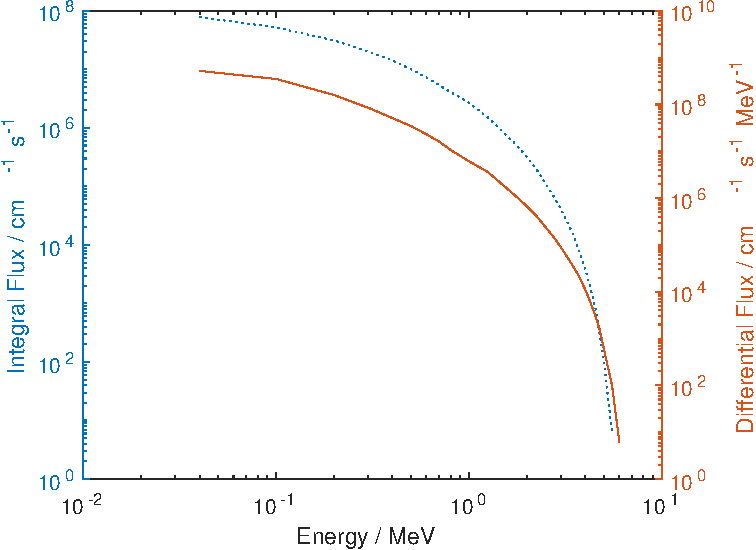
\includegraphics[width=\textwidth]{Media/E_Electron_Flux}
         \caption{Average spectra of trapped electrons around Earth}
         \label{fig:trappedelectronsEarth}
     \end{subfigure}
     \hfill
     \begin{subfigure}[b]{0.49\textwidth}
         \centering
         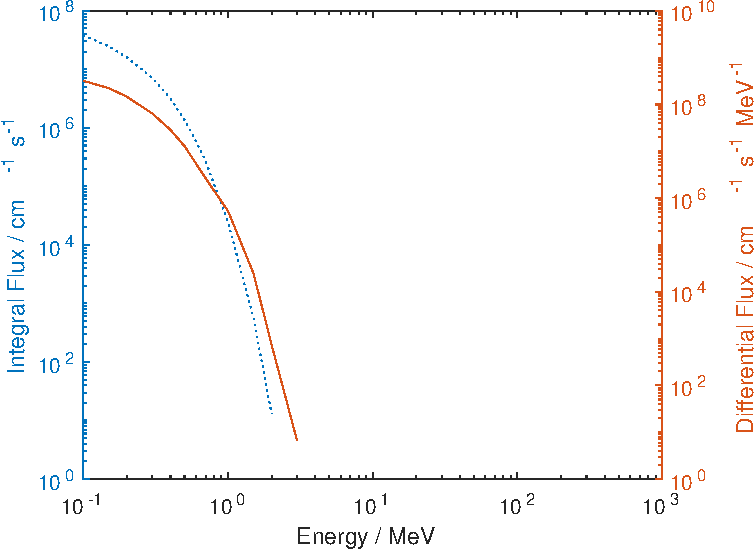
\includegraphics[width=\textwidth]{Media/E_Proton_Flux}
         \caption{Average spectra of trapped protons around Earth}
         \label{fig:trappedprotonsEarth}
     \end{subfigure}
     \hfill
     \begin{subfigure}[b]{0.49\textwidth}
         \centering
         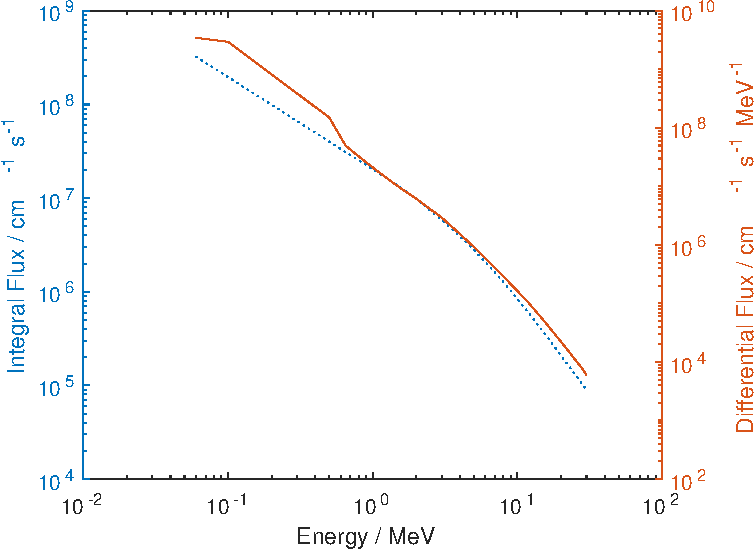
\includegraphics[width=\textwidth]{Media/J_Electron_Flux}
         \caption{Average spectra of trapped electrons around Jupiter}
         \label{fig:trappedelectronsJupiter}
     \end{subfigure}
     \hfill
     \begin{subfigure}[b]{0.49\textwidth}
         \centering
         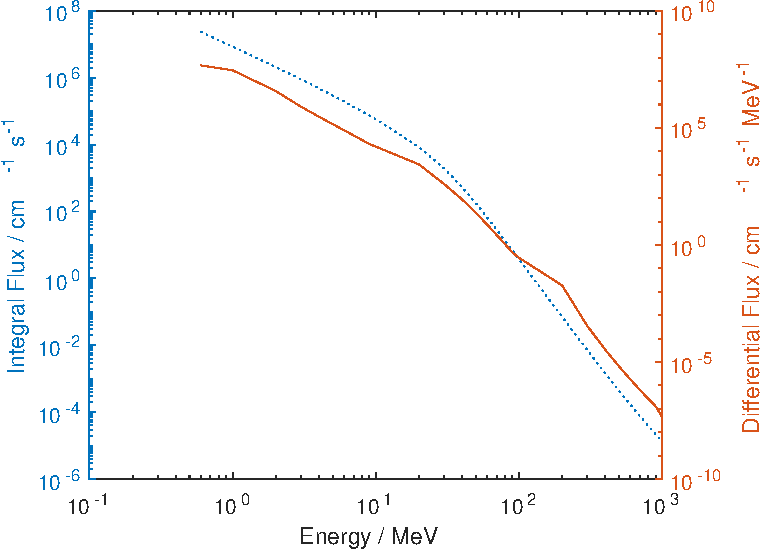
\includegraphics[width=\textwidth]{Media/J_Proton_Flux}
         \caption{Average spectra of trapped protons around Jupiter}
         \label{fig:trappedprotonsJupiter}
     \end{subfigure}
     \caption{Average trapped proton and electron fluxes on an orbit around earth at 25,000 km, through the outer Van Allen radiation belt, and on Europa's orbit around Jupiter.}
     \label{fig:trappedprotonelectronfluxes}
\end{figure}

\clearpage

\subsection{Radiation Exposures}

\label{subsec:AppendixRadiationExposures}

In order to simulate the TID for different radiation protections the Geant4 tool Multi-Layered Shielding Simulation (MULASSIS) is used. As target material silicon is selected with a thickness of 1 \(\mu \text{m}\). As shape a planar slap is selected because of the ice ground on one side of the rover.

\begin{figure}[htb]
     \centering
     \begin{subfigure}[b]{0.49\textwidth}
         \centering
         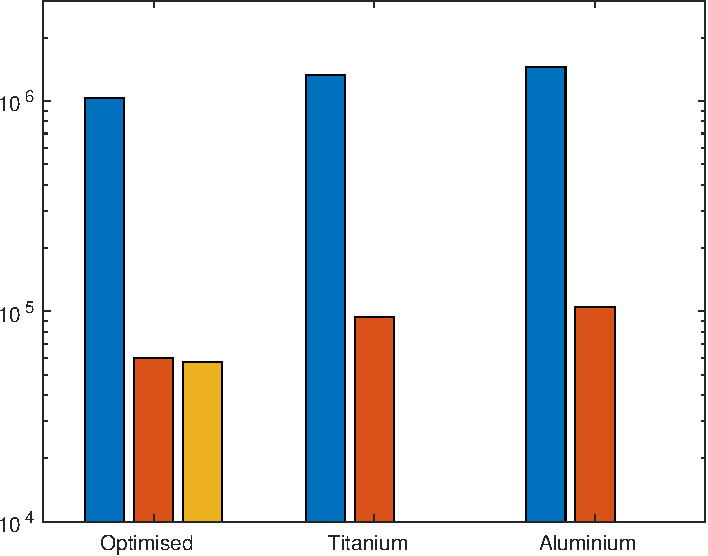
\includegraphics[width=\textwidth]{Media/J_Electron_Shielding}
         \caption{TID for Electrons as Source Particles}
         \label{fig:TIDElectronShielding}
     \end{subfigure}
     \hfill
     \begin{subfigure}[b]{0.49\textwidth}
         \centering
         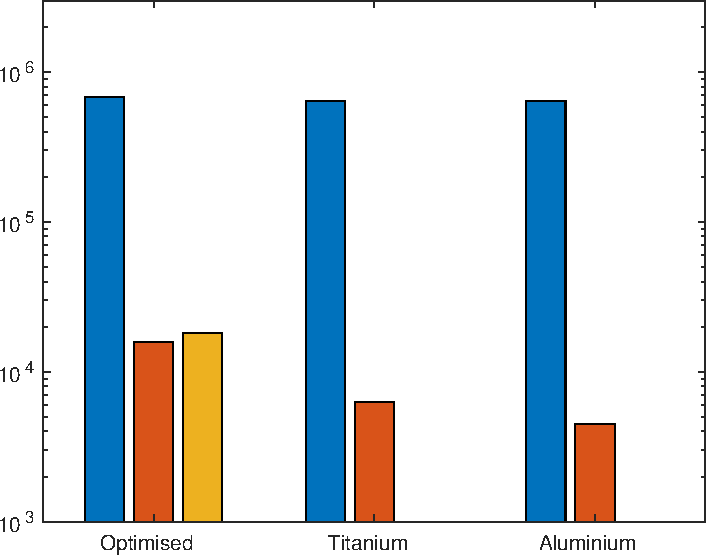
\includegraphics[width=\textwidth]{Media/J_Proton_Shielding}
         \caption{TID for Protons as Source Particles}
         \label{fig:TIDProtonShielding}
     \end{subfigure}
     \caption{TID of aluminium, titanium, and the optimised radiation structure shown in \autoref{tab:OptimalRadiationProtection} with a weight target of all three structures of 0.5 \(\text{g/cm}^2\) over 30 days of exposure on Europa.}
     \label{fig:AluminiumTitanOptimised}
\end{figure}

\begin{table}[htb]
\centering
\caption{Used components and the respective radiation tolerance and location}
\begin{adjustbox}{max width=\textwidth}
\begin{tabular}[l]{lccccc}

	\toprule
		Components	&	Rated TID	&	Exposed TID	&	Location\\
	\midrule
	
	BLDC Motors	&	-	&	< 205	&	locomotion housing\\	
	
	Stepper Motors	&	100 000	&	< 205	&	locomotion housing\\
	
	Harness	&	-	&	< 98	&	chassis\\	
	
	Stereo Vision Cams	&	40	&	< 31	&	camera housing\\	
	
	OBC	&	1 000	&	< 17	&	E-Bay\\
	
	PCDU	&	20	&	< 17	&	E-Bay\\
	
	Transmitter	&	20	&	< 17	&	E-Bay\\
	
	Receiver	&	20	&	< 17	&	E-Bay\\
	
	Battery	&	20	&	< 17	&	E-Bay\\
	
	Housekeeping Board	&	\(\approx\) 20	&	< 17	&	E-Bay\\
	
	IMU	&	\(\approx\) 20	&	< 17	&	E-Bay\\
	
	Multiplexer	&	\(\approx\) 20	&	< 17	&	E-Bay\\
	
	Ground Radar	&	\(\approx\) 20	&	< 17	&	E-Bay\\
	
	Sun Sensor	&	10 000	&	2 000	&	outside rover\\
	
	Camera Lenses	&	10 000	&	2 000	&	outside rover\\

	\bottomrule

\end{tabular}
\end{adjustbox}
\label{tab:RadiationList}
\end{table}

\begin{figure}[htb]
     \centering
     \begin{subfigure}[b]{0.49\textwidth}
         \centering
         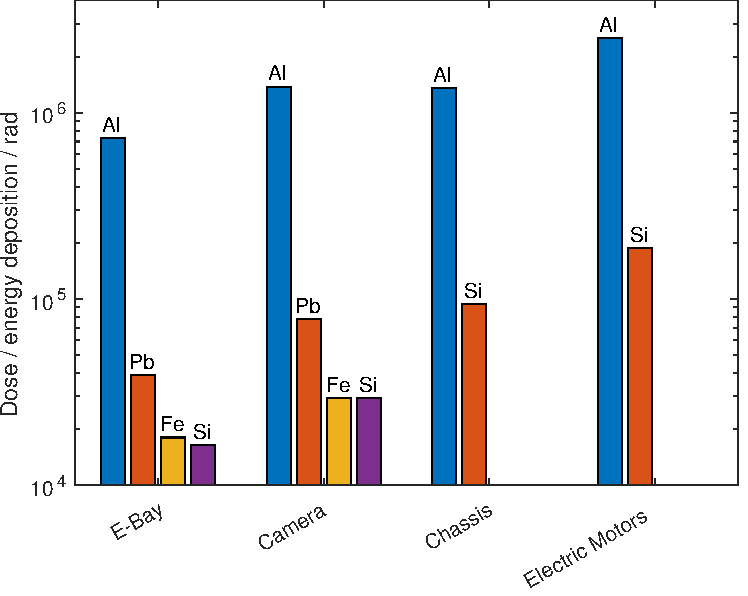
\includegraphics[width=\textwidth]{Media/J_Electron_Compartments}
         \caption{TID for Electrons as Source Particles}
         \label{fig:TIDElectronShielding}
     \end{subfigure}
     \hfill
     \begin{subfigure}[b]{0.49\textwidth}
         \centering
         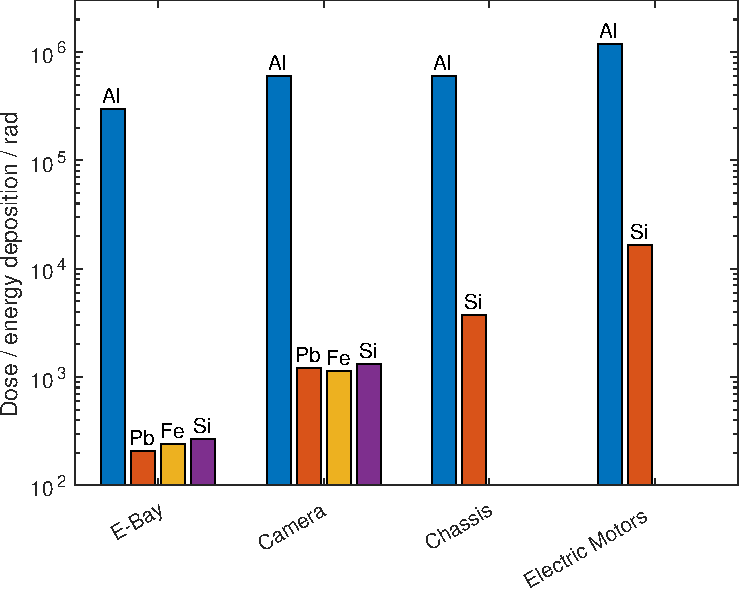
\includegraphics[width=\textwidth]{Media/J_Proton_Compartments}
         \caption{TID for Proton as Source Particles}
         \label{fig:TIDProtonShielding}
     \end{subfigure}
     \caption{TID for different compartments as seen in \autoref{fig:RadiationOverview}. The E-Bay is shielded by 4 mm aluminium, 0.415 mm lead, and 0.033 mm iron; the camera compartment by 2 mm aluminium, 0.415 mm lead, and 0.033 mm iron; the chassis by 2 mm aluminium; the electric motors by 1 mm aluminium.}
     \label{fig:CompartmentTID}
\end{figure}

\newpage

\subsection{Improvements}

\label{app:AppendixRadiationImprovements}

All simulations of the improvements introduced in \autoref{subsec:RadiationImprovements} are performed in the same way as in \autoref{subsec:AppendixRadiationExposures}. \\ \\
In \autoref{fig:Radiation_Improvements_Individual}, the TID over 30~days within the E-Bay is shown with only the aluminium structure. If all components with a radiation resistance under 43.27~krad are shielded individually, the additional shielding structure around the E-Bay can be removed and the aluminium structure would be sufficient. \\ \\
The aluminium structure would also be sufficient if a layer of 1~cm of water mined in-situ would be used as shielding which is present in \autoref{fig:Radiation_Improvements_Ice}. \\ \\
Both improvements would save the mass of the lead and iron shielding for the optimised shielding of 897.2~g.

\begin{figure}[htp]
	\centering
	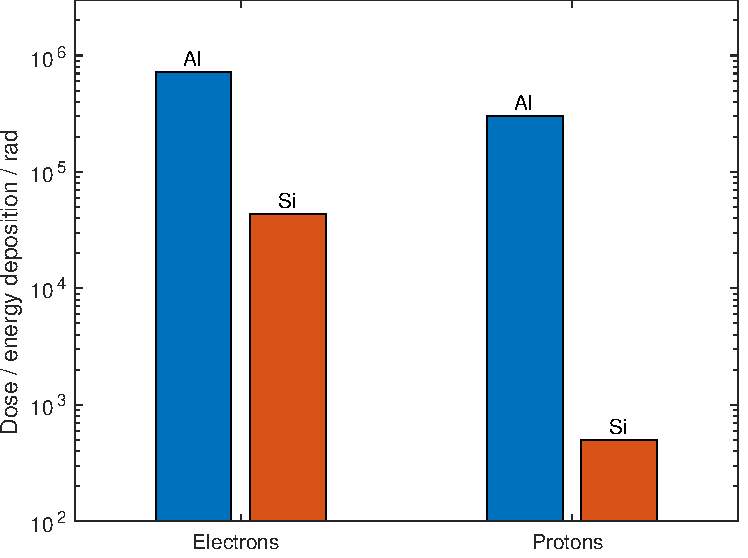
\includegraphics[width=0.7\textwidth]{Media/J_Improvements_Individual}
	\caption{TID with 4 mm Al shielding over a mission duration of 30 days}
	\label{fig:Radiation_Improvements_Individual}
\end{figure}

%The resulting mass savings can be calculated with \autoref{eq:RadiationImprovementsIndividual} with \(m^*\) as the specific weight of the radiation protection and \(N\) as the amount of components within the E-Bay with a radiation resistance under 43.27~krad as of \autoref{tab:RadiationList}.

%\begin{equation}
%	\Delta m = SA_\text{E-Bay} \cdot m^*_\text{Shielding} - \sum\nolimits_{n=0}^N SA_\text{Component, n} \cdot m^*_\text{Shielding}
%	\label{eq:RadiationImprovementsIndividual}
%\end{equation}

%With inserted values this results in a mass saving of \(\Delta m\) = 736.2~g.

\begin{figure}[htp]
	\centering
	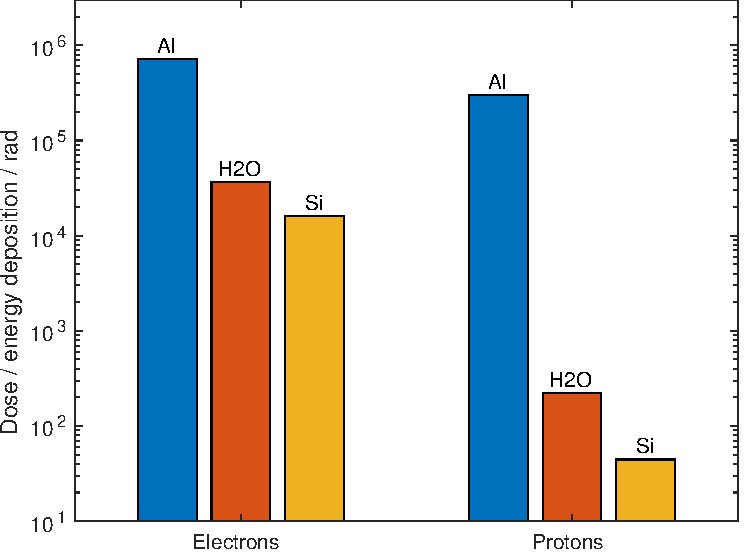
\includegraphics[width=0.7\textwidth]{Media/J_Improvements_Ice}
	\caption{TID with 4 mm Al shielding and 1 cm of Water over a mission duration of 30 days}
	\label{fig:Radiation_Improvements_Ice}
\end{figure}

\clearpage

\setcounter{figure}{0}
\setcounter{table}{0}

%-----------------------------------------------------------
\section{Digital Appendix}		\label{app:DigitalAppendix}
%-----------------------------------------------------------

\begin{table}[htb]
	\centering
	\begin{tabular}{llcc}
	\toprule
		Name  & Path & Type & Size  \\
	\midrule
		TCS Analysis final & 300 Thermal\ & Exle Sheet with Macros, *.xlsm & 189 kB  \\
	\bottomrule
	\end{tabular}
	\caption{Digital Appendix}
	\label{app:DigitalAppendix}
\end{table}

\cleardoublepage